\documentclass[UTF8]{ctexart}
\usepackage{booktabs}
\usepackage{graphicx}
\usepackage[final]{pdfpages}
\usepackage[stable]{footmisc}
\usepackage{threeparttable}
\usepackage{indentfirst}
\setlength{\parindent}{0pt}

\usepackage{minted}
\usepackage{listings}
\usepackage{xcolor}
\lstset{
    rulesepcolor= \color{gray},
    breaklines=true,
    numbers=left,
    numberstyle= \small,
    commentstyle=\color{gray},
    frame=shadowbox
}
\usepackage{subfigure}

\title{基于Android/Java处理机调度算法模拟实现}
\author{软件工程2003杜睿}
\date{}

\begin{document}
\tableofcontents
\maketitle

\section{设计目的}
CPU是计算机系统的重要资源,处理机调度是操作系统的核心内容。进程调度和作业调度作为处理机调度的重要组成部分,其调度算法优劣直接影响操作系统的性能好坏。模拟设计进程调度和作业调度算法,在掌握各种调度算法的同时,可以进一步加深理解处理机管理技术的原理及特点。

\section{系统设计}

\subsection{设计任务\footnote{基于《2020级操作系统课程设计任务书》,2023年1月,有删节}}

\begin{enumerate}
    \item 可任意选择作业(进程)数量、作业(进程)优先级、作业提交时间(进程到达时间)和预计运行时间。
    \item 模拟实现作业调度中先来先服务(FCFS)、短作业优先(SJF)和最高响应比调度(HRRN)算法。每次作业调度时,显示各作业的执行情况(开始执行时间,结束时间,周转时间);最后,计算并列出平均周转时间并对相同情况下不同调度算法进行性能分析比较。
    \item 模拟实现进程调度中基于优先级的时间片轮转调度算法(PRR)和多级反馈队列轮转调度算法(MFQ)。每次进行进程切换时,显示各进程执行情况(剩余时间,进程状态,进程排队情况),最后列出各进程的开始执行时间和结束时间。
\end{enumerate}

\subsection{任务分析}

一个作业从用户提交开始到占有处理机被执行,一般来要由系统三级调度才能实现,即作业调度、内存调度、进程调度。其中最为重要的:
\begin{description}
    \item[作业调度] 主要是完成作业\footnote{用户向计算机提交任务的任务实体,《计算机操作系统教程(第四版)》,清华大学出版社}从\emph{后备状态}到\emph{可执行状态}的转变,即按照某原则,从\emph{外存后备队列}中挑选作业,将其装入\emph{内存}并为其创建进程;
    \item[进程调度] 主要是完成进程从\emph{就绪状态}到\emph{执行(完成)状态}的转变,即按照某策略,从\emph{内存就绪队列}中选取进程,为其分配处理机使其运行。
\end{description}

\begin{table}[htbp]
    \caption{常用的处理机调度策略}
    \centering

    \begin{threeparttable}
        \begin{tabular}{cccccc}
            \toprule
            算法名称           & 主要适用范围       & 默认调度方式         \\
            \midrule
            先来先服务         & 作业调度\&进程调度 & 非抢占式             \\
            短作业(进程)优先 & 作业调度\&进程调度 & 非抢占式             \\
            高响应比优先       & 作业调度           & 非抢占式             \\
            时间片轮转         & 进程调度           & 抢占式(不抢时间片) \\
            多级反馈队列       & 进程调度           & 抢占式(抢占时间片) \\
            \bottomrule
        \end{tabular}

        \zihao{-6}
        \begin{tablenotes}
            \item [*]   调度策略也就是调度算法
        \end{tablenotes}

    \end{threeparttable}
    \qquad
\end{table}

基于设计内容要求及上述理论常识,可以做出如下基本假设:
\begin{enumerate}
    \item 作业调度和进程调度是互补共存的层级关系。不考虑内存调度的前提下,实现任何算法,至少要实现两级调度:作业调度及进程调度。
    \item 作业和进程可以合二为一,统一抽象为任务\footnote{作业是提交层面的任务,进程是执行层面的任务,作者注}。不考虑阻塞的前提下,一个任务大致可归为未提交态、收容态、就绪态、运行态及销毁态。
    \item 调度是种将何资源分配给何任务的决策行为。从各级调度的交互上说,调度可以分为:本级进行调度、移交上层调度及委托下层调度。
\end{enumerate}

综上,我对《任务书》要求的系统设计内容进行重述:\emph{通过编程,模拟实现一个单(多)道批处理系统及其多级调度策略,输入作业序列,输出作业进入内存的时间、结束时间、平均周转时间,展示各作业的执行时间线。}

任务书中要求的原任务与多级调度实现的对应关系如下:
\begin{table}[htbp]
    \caption{批处理系统的多级调度明细}
    \centering
    \begin{tabular}{cccc}
        \toprule
        原任务*                    & 作业调度   & 进程调度   & 内存限制 \\
        \midrule
        先来先服务                 & *          & 先来先服务 & 1        \\
        短作业优先                 & *          & 先来先服务 & 1        \\
        高响应比优先               & *          & 先来先服务 & 1        \\
        \midrule
        基于动态优先级的时间片轮转 & 先来先服务 & *          & INF      \\
        多级反馈队列               & 先来先服务 & *          & INF      \\
        \bottomrule
    \end{tabular}
    \qquad
\end{table}

\subsection{概要设计} \label{v0}

要模拟批处理系统,就须要模拟时钟、任务及其状态、分级调度。

\begin{description}
    \item[时钟] 标定时间流逝的基准,以便执行作业调度、进程调度、性能分析等。每流逝一个单位时间,系统至少要进行一次调度。所以,可以建立“时钟”与“调度器”之间的依赖关系,当时钟发生改变时应该自动通知调度器,调度器接受信息并做出响应。时钟,被称为观察目标;调度器,被称为观察者。一个观察目标可以对应对个观察者,可以根据需要增加和删除观察者。这种设计模式被称为\emph{观察者模式}或\emph{发布-订阅模式}。
    \item[任务] 每个任务都有提交时间、到达时间等属性;运行中任务的剩余时间随时间流逝而减少(从这种意义说,运行中的进程应当观察时间流逝,并自主改变剩余时间字段)。

        任务揉杂作业和进程,集成两者的属性,
        即id、优先级、状态、时钟,提交时间、预计需要时间,到达时间、开始时间、剩余时间、完成时间。

        在模拟逻辑上,状态包含五种类型:未提交、收容、就绪、运行、结束。未提交,代表用户输入作业序列中的提交时间晚于当前时钟时刻;收容,代表作业已提交,进入外存收容队列(外存一般没有容量限制);就绪,代表进程已创建,进入内存就绪队列(内存一般有容量限制);运行,代表进程获得处理机资源,随时间流逝剩余时间递减。
    \item[调度] 任务状态由调度器进行切换;调度是分层级的。

        作业提交与调度细节应当是解耦的,同时为较好地实现“分级”调度,可以将调度器链式组织,各司其职,又保证了作业在各级调度中的传递,直到进程销毁并记录日志。这种思想来源于\emph{职责链模式}。

    \item[机器] 整合时钟、任务、调度,并接受测试样例或用户输入,输出日志。不同的调度策略在各层级上排列组合,可以衍生出多种具体“机器”。为将对象创建和对象使用解耦,可以使用\emph{工厂方法模式}。
\end{description}

\begin{figure}[htbp]
    \centering
    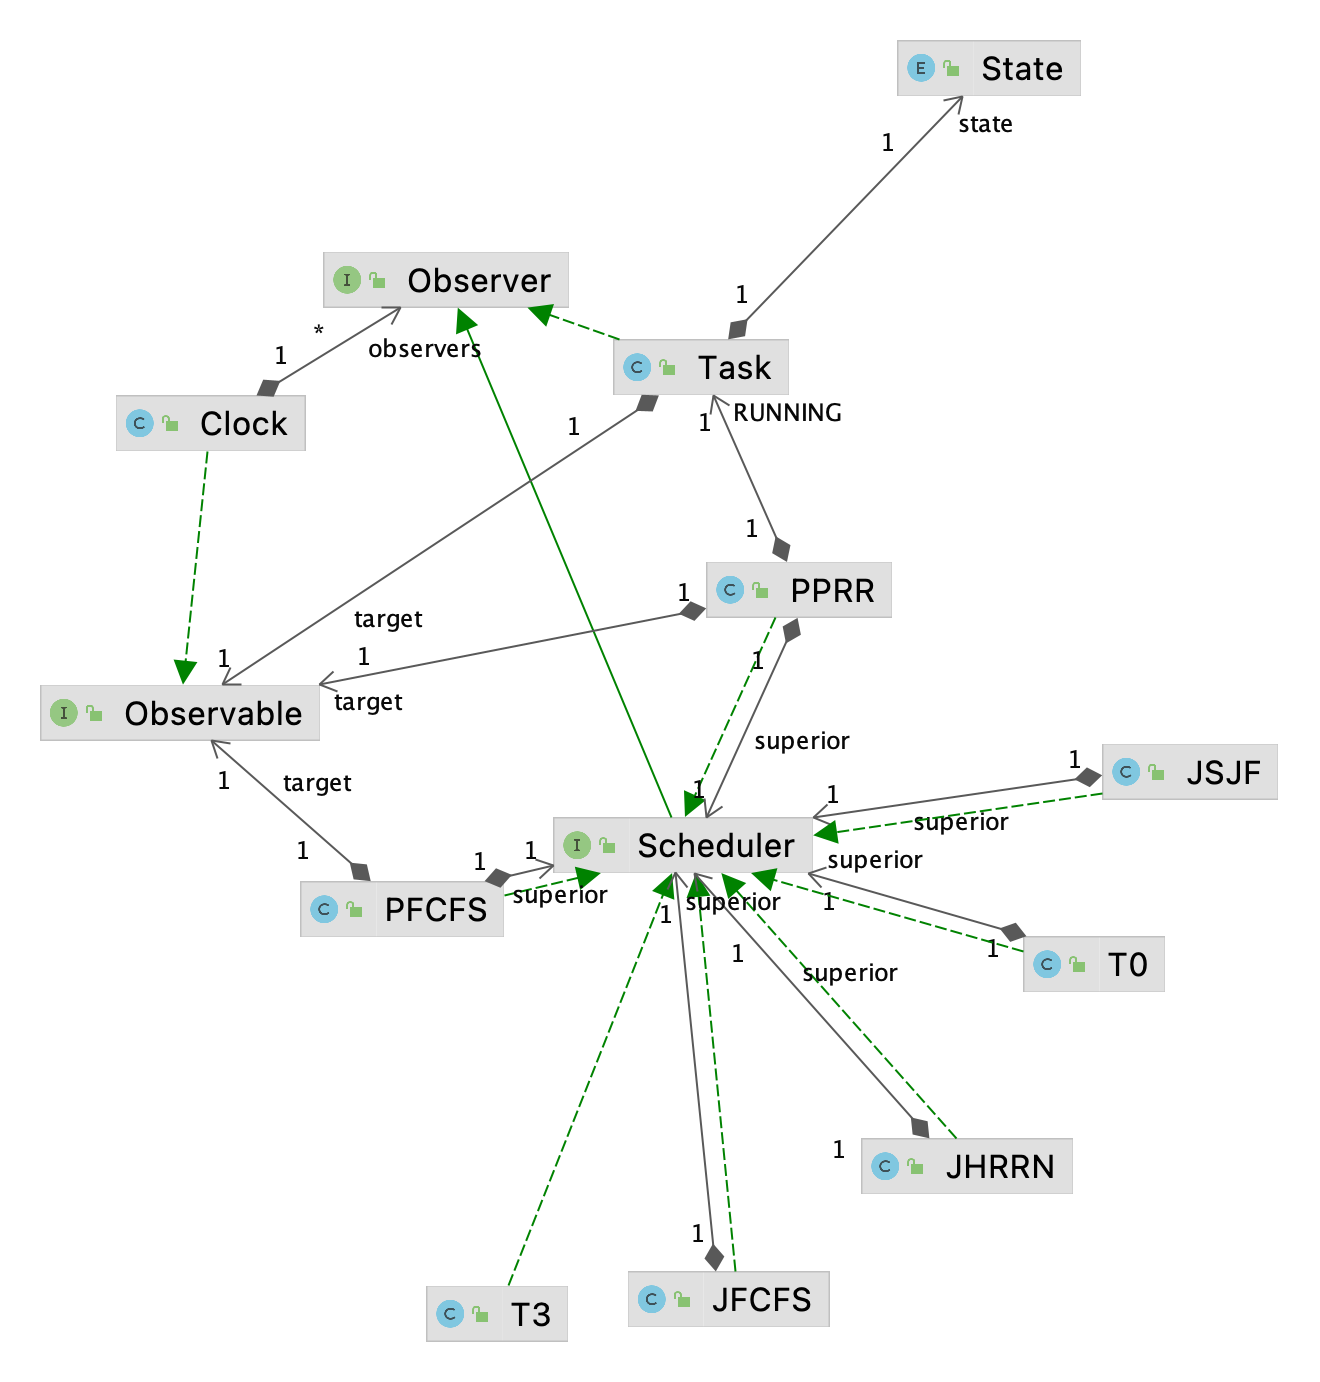
\includegraphics[height=395pt]{v0-class-compat.png}
    \caption{UML类图(第一版)}
\end{figure}

\newpage
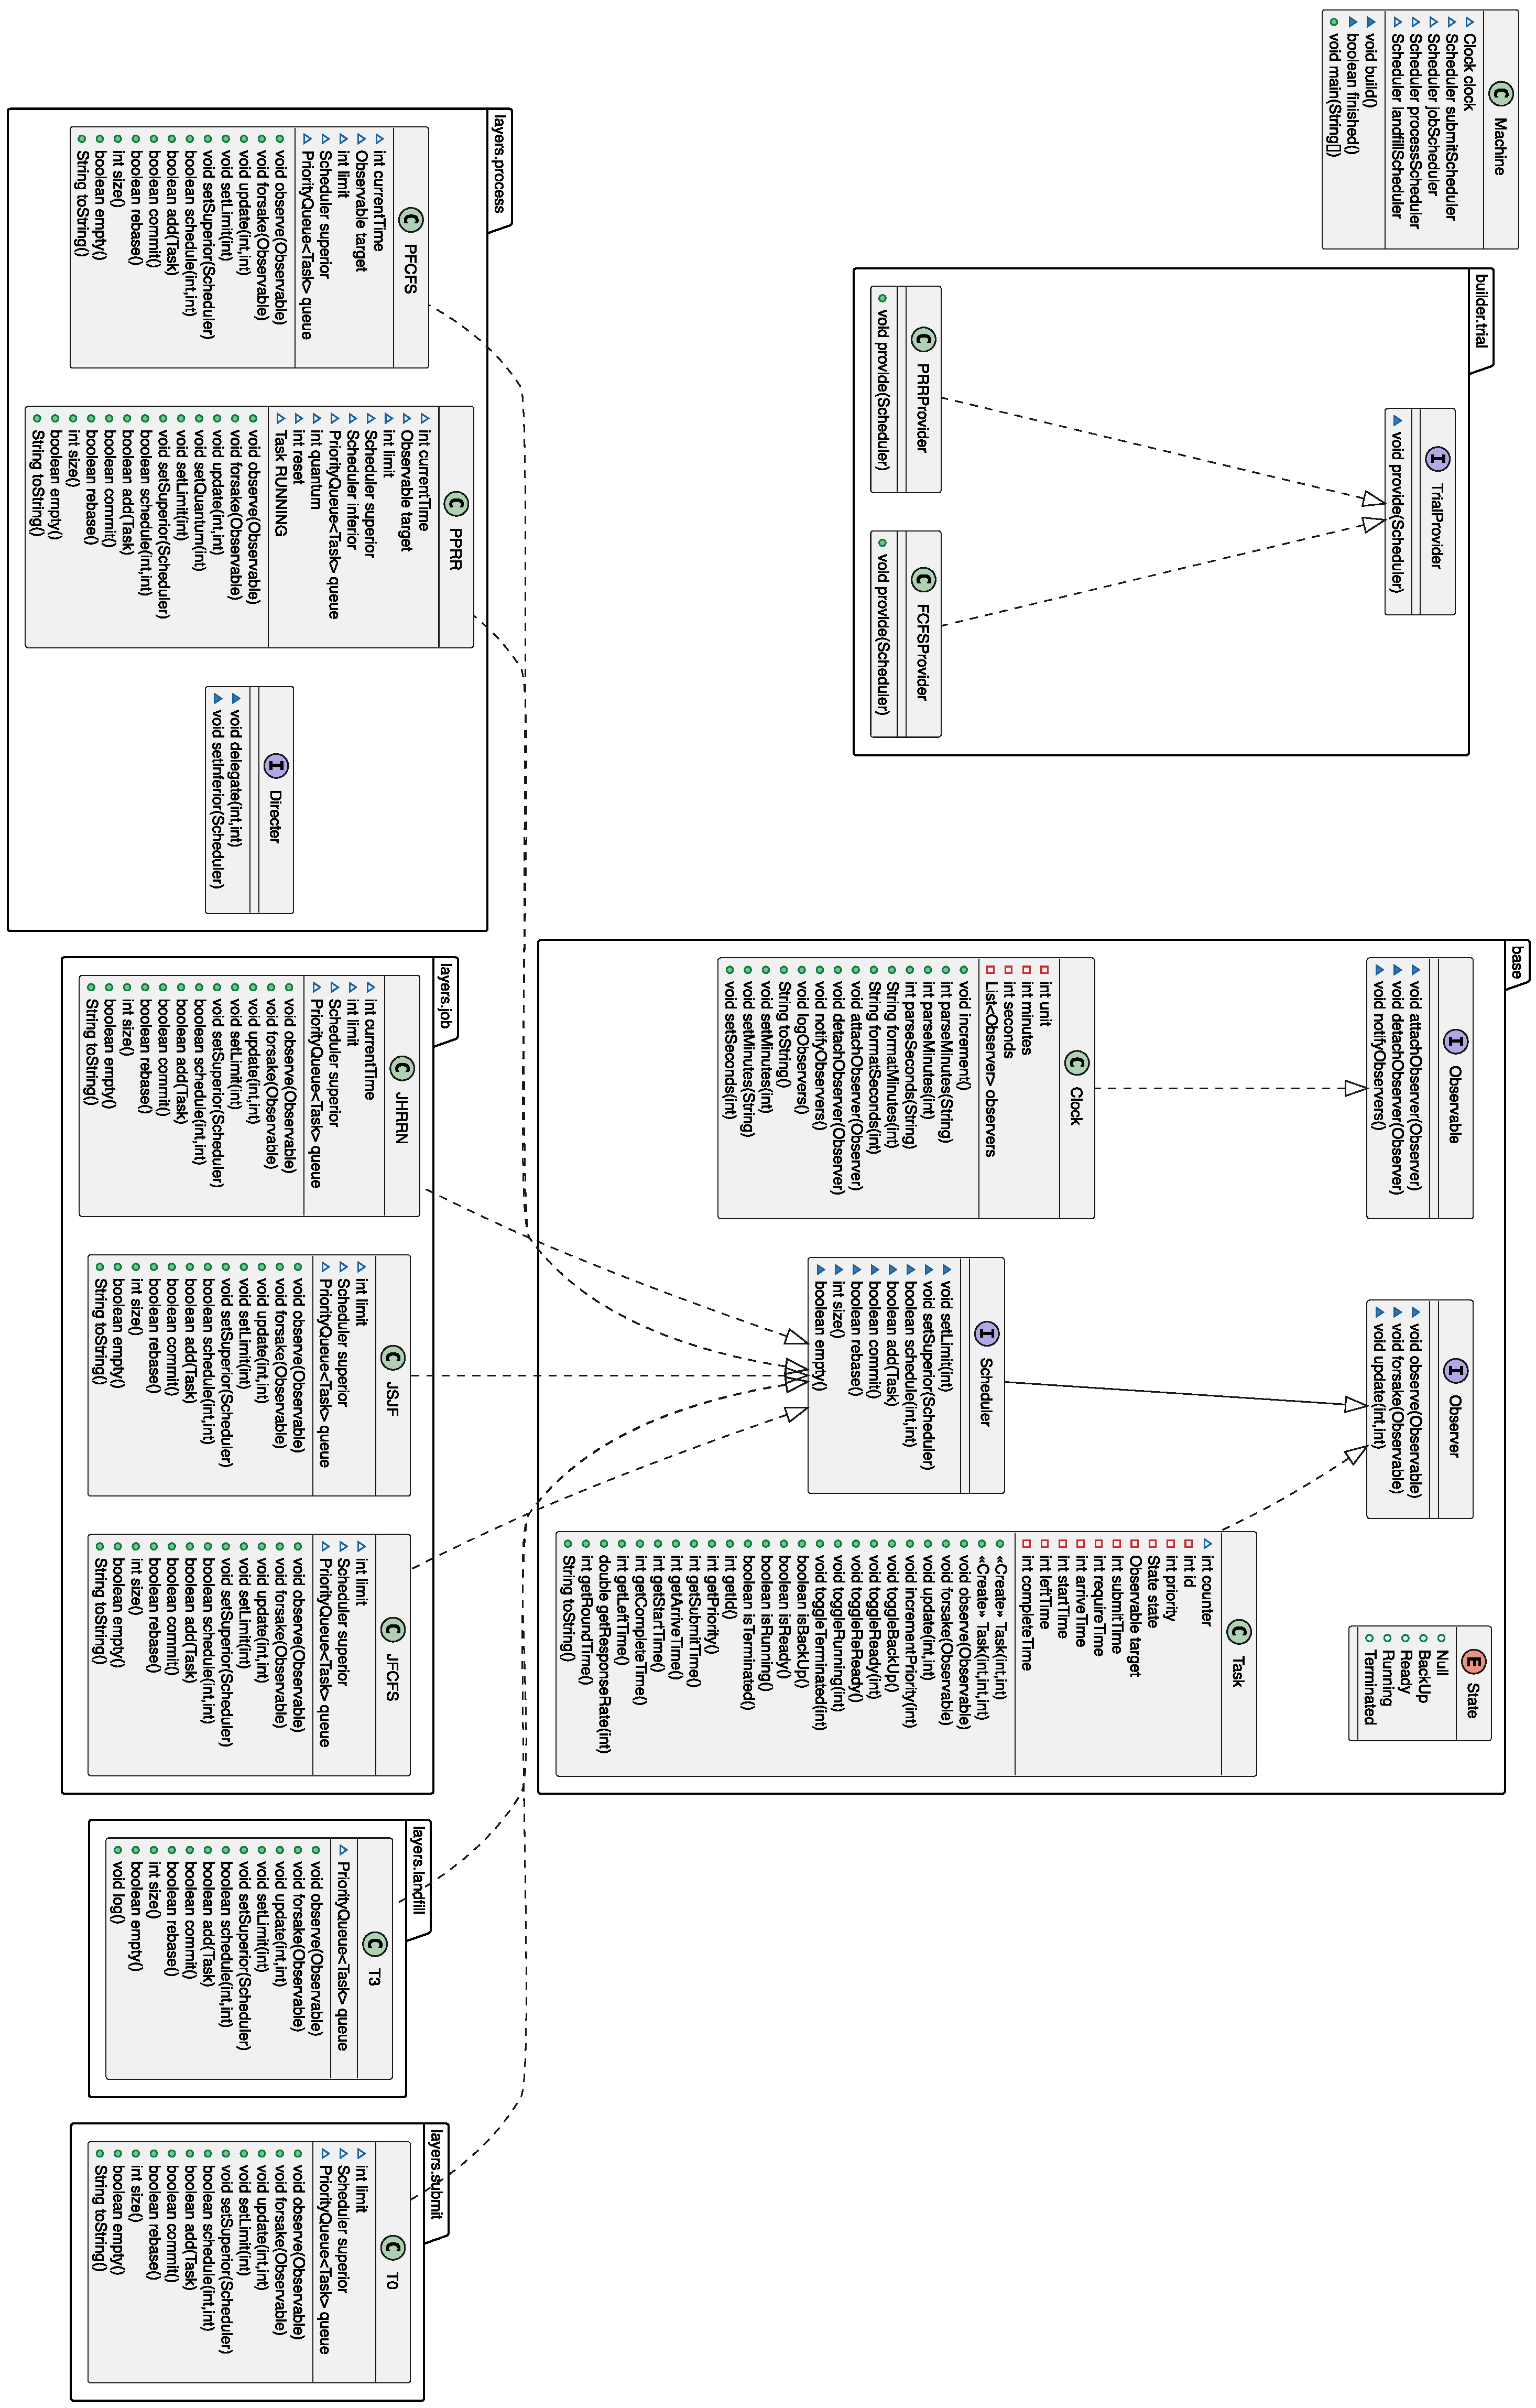
\includepdf{v0-class.pdf}
\newpage

\subsection{质量评审}

基于 \ref{v0} 实现的系统,将存在一个致命缺陷:延时。之所以会延时,主要是因为各个时间观察者对于时间流逝的感知顺序是固定、单向的。
\begin{figure}[htbp]
    \centering
    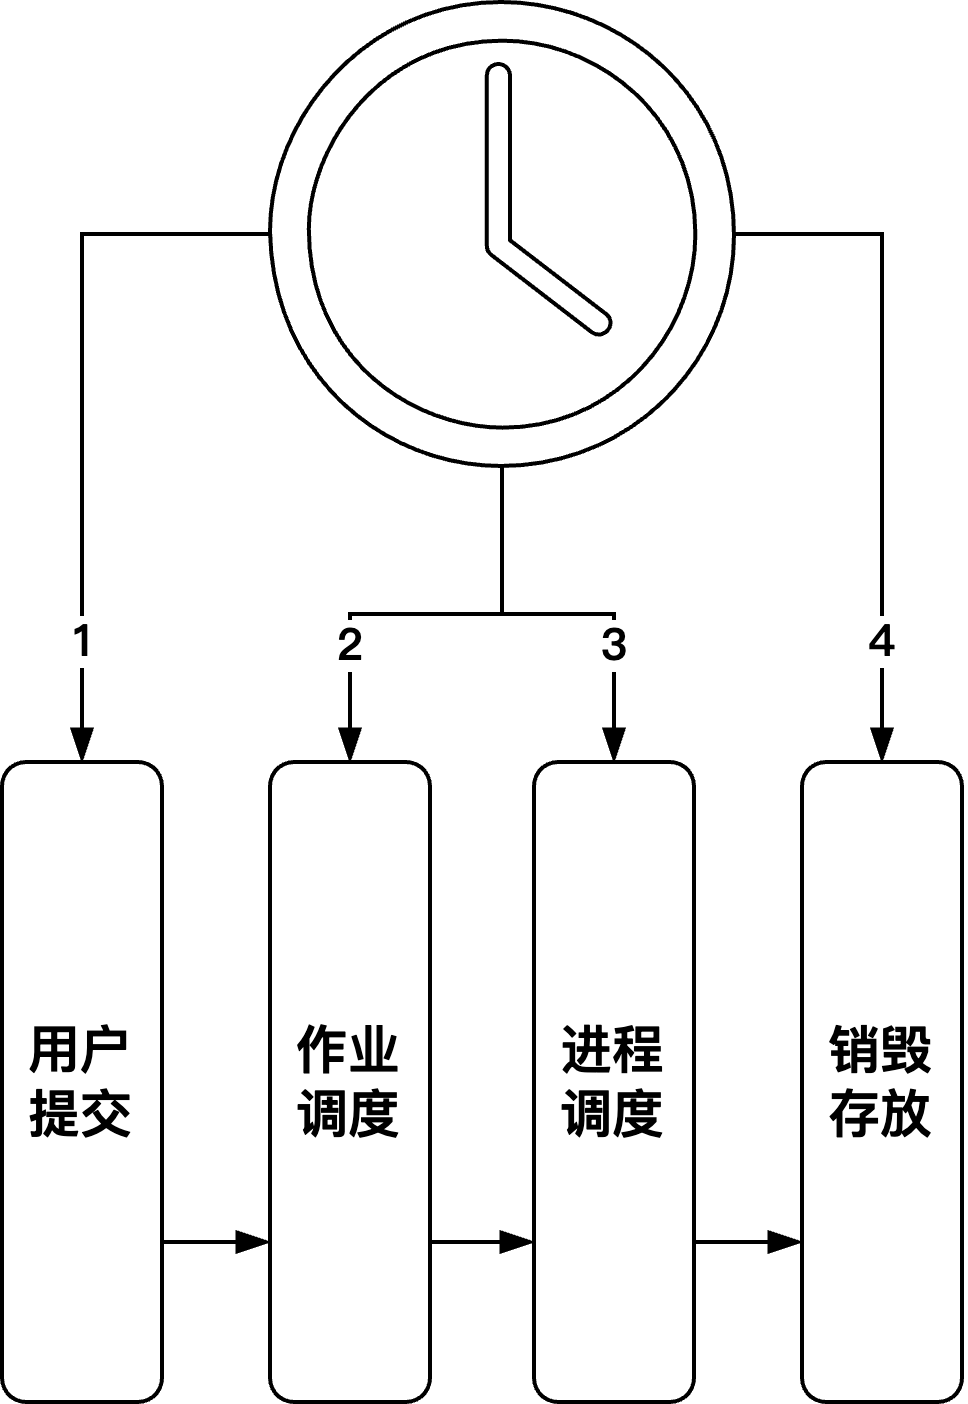
\includegraphics[height=13.2em]{i-lag.png}
    \caption{通知顺序}
\end{figure}

虽然从层级上说,作业调度高于(先于)进程调度,但是从顺序上说,在单位时间流逝后,有可能出现先作业调度、再进程调度、再作业调度的情况。

\begin{table}[htbp]
    \caption{错误案例(单道批处理系统)}
    \centering
    \begin{tabular}{cccccc}
        \toprule
        时刻   & 收容队列            & 就绪队列            & 备注                 \\
        \midrule
        09:59  & \{\}                & \{[运行,余1分钟]\} & 初始状态             \\
        10:00  & \{\}                & \{[运行,余1分钟]\} & 用户提交新作业       \\
        10:00  & \{[收容,余1分钟]\} & \{[运行,余1分钟]\} & 内存已满|无作业调度 \\
        10:00  & \{[收容,余1分钟]\} & \{[运行,余1分钟]\} & 正在运行|无进程调度 \\
        10:00  & \{[收容,余1分钟]\} & \{[结束,余0分钟]\} & 进程自主修改剩余时间 \\
        \bottomrule
        10:01  & \{[收容,余1分钟]\} & \{[结束,余0分钟]\} & 内存已满|无作业调度 \\
        10:01  & \{[收容,余1分钟]\} & \{\}                & 释放进程(进程调度) \\
        \bottomrule
        10:02  & \{\}                & \{[就绪,余1分钟]\} & 掉入内存(作业调度) \\
        10:02  & \{\}                & \{[运行,余1分钟]\} & 运行进程(进程调度) \\
        10:02  & \{\}                & \{[结束,余0分钟]\} & 进程自主修改剩余时间 \\
        \ldots & \ldots              & \ldots              & \ldots               \\
        \bottomrule
    \end{tabular}
    \qquad
\end{table}

本错误案例中,10:00~10:01处理机竟然处于空闲状态。这是因为:
\begin{itemize}
    \item 进程运行不受进程调度控制,进程调度没有及时将结束进程向上提交;
    \item 进程调度即使向上提交,作业调度也无法预知未来,并为其创建进程。
\end{itemize}

下面提出两种可能的改进方案,并加以分析:
\begin{description}
    \item [调整时间单位] 承认并接受延时的存在,并将时间继续细分。例如,倘若单位设定为“秒”,那么在“分钟”维度上看,延时仿佛并不存在。不过,只要没有无限细分,延时累积最终必将影响结果。
    \item [优化通信机制] 扭转各层对时间流逝固定、单向的感知顺序。拟人地说,各层消息传递机制不能只包含“向上告知”,还要包含“向下问责”。进程调度结束后,倘若可以通知作业调度:“你那里还有什么要我签字处理的吗?”;那么,延时问题说不定就可以迎刃而解。
\end{description}

\section{系统实现}

\subsection{核心实现}
在上一节的基础上,添加以下前提假设,以便系统实现:时钟的最小颗粒单位为分钟,所有作业均在23:59前提交并结束。《任务书》设计描述中,单位并不统一,如,“进程到达时间(单位时间)”、“作业提交时间(时钟时刻)”、“预计运行时间(小时)”。所以需要在正式输入核心部分前,需要进行数据预处理和单位标准化。

以“多级队列反馈队列”为例,我们需要实现(类图见下页):
\begin{itemize}
    \item 核心组件:
          \begin{itemize}
              \item 任务、状态
              \item 时钟(观察对象)
              \item 提交“调度”、作业调度、进程调度、销毁“调度”(严格意义上说,提交和销毁不属于调度,它们是对定时提交和进程销毁的一种模拟)
          \end{itemize}
    \item 边缘组件:
          \begin{itemize}
              \item 处理机工厂,用不同算法构建各级调度
              \item 测试样例工厂,创建任务并添加至提交“调度”
          \end{itemize}
\end{itemize}

\begin{figure}[htbp]
    \centering
    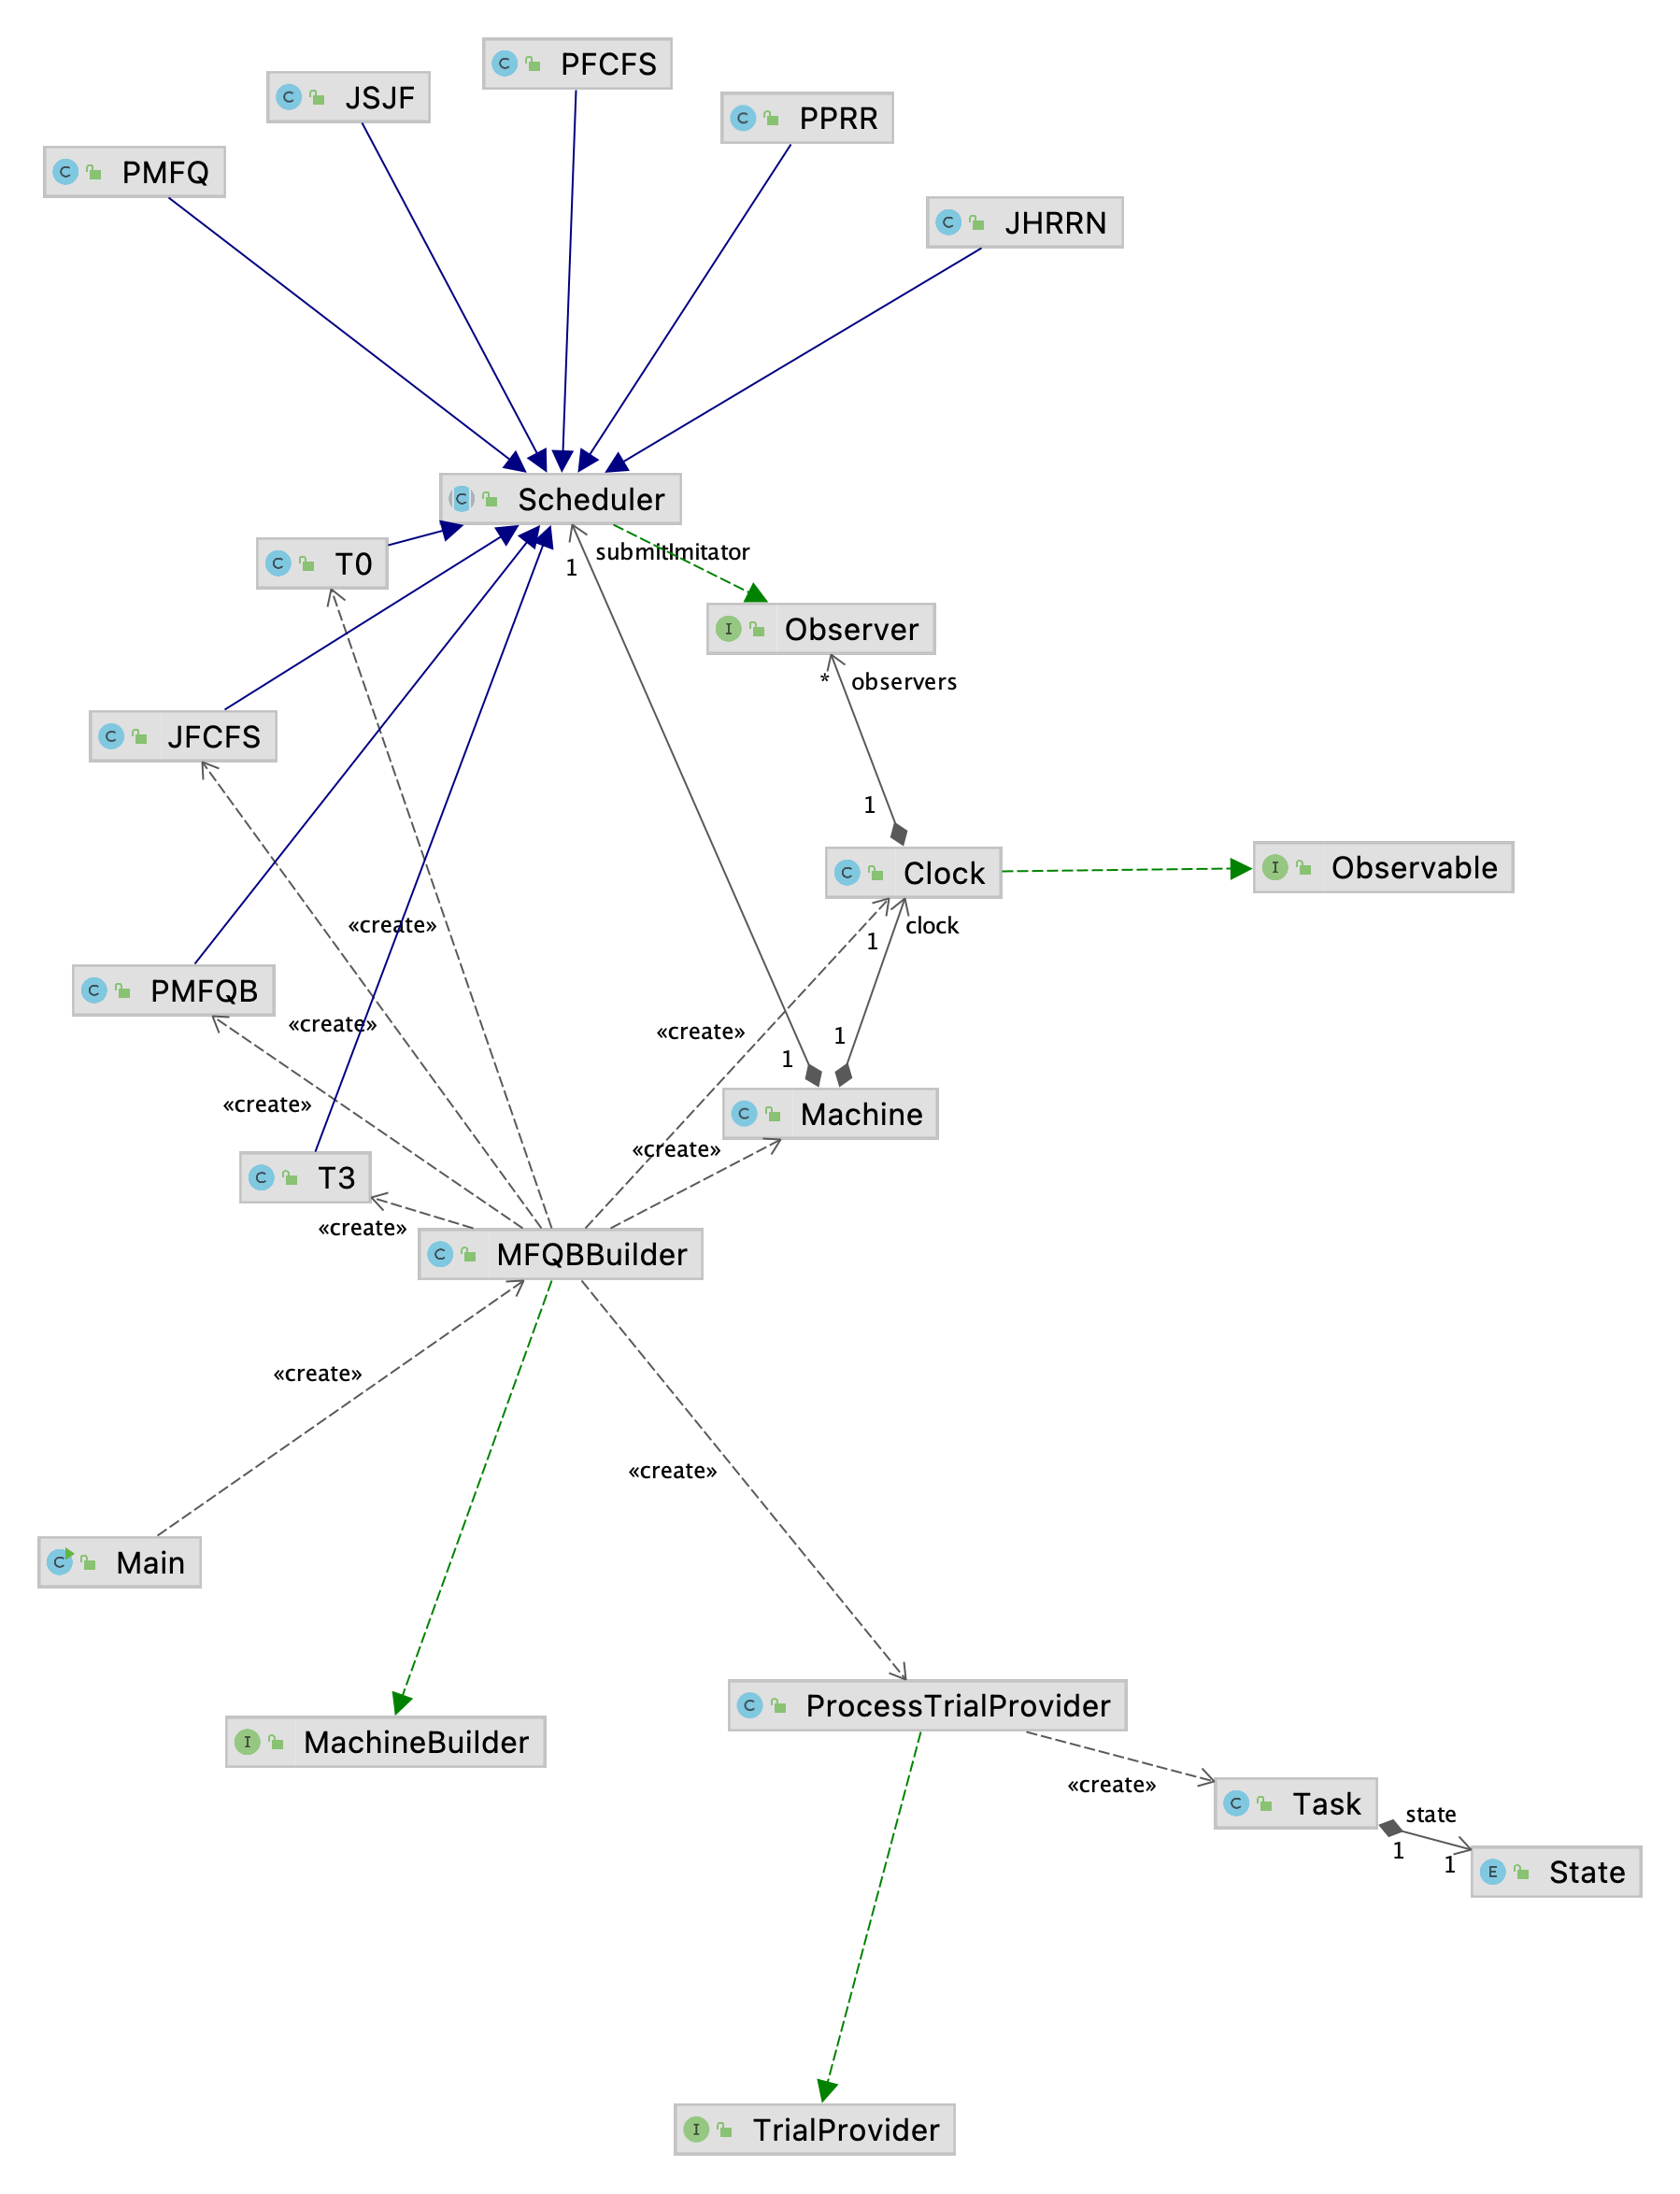
\includegraphics[height=550pt]{v1-class-compat.png}
    \caption{UML类图(第二版)}
\end{figure}

多级调度各司其职,共同作为批处理系统的重要组成部分发挥作用:

\begin{table}[htbp]
    \caption{常用的处理机调度策略}
    \centering

    \begin{threeparttable}
        \begin{tabular}{cccccc}
            \toprule
            多级调度 & 调度方式                                    & 调度时机                 & 调度次序 & 任务状态   \\
            \midrule
            用户提交 & $\uparrow$                                  & 提交时刻 $\leq$ 当前时刻 & 提交时间 & 未提交     \\
            作业调度 & $\uparrow$                                  & 时间流逝 \& 上层命令     & *        & 收容       \\
            进程调度 & $\uparrow$、$\leftrightarrow$、$\downarrow$ & 时间流逝                 & **       & 就绪、运行 \\
            进程销毁 &                                             &                          &          & 销毁       \\
            \bottomrule
        \end{tabular}

        \zihao{-6}
        \begin{tablenotes}
            \item [1]   $\uparrow$移交上层调度,$\leftrightarrow$本层级调度,$\downarrow$、委托下层调度
            \item [2]   * 提交时间、剩余时间、响应比
            \item [3]   ** 优先级(多级队列优先次序)
        \end{tablenotes}

    \end{threeparttable}
    \qquad
\end{table}

\subsubsection{作业调度}
实现单道批处理系统,作业调度分别使用“先来先服务算法”、“短作业优先算法”、“高响应比优先算法”,进程调度统一使用“先来先服务算法”。

\begin{figure}[htbp]
    \centering
    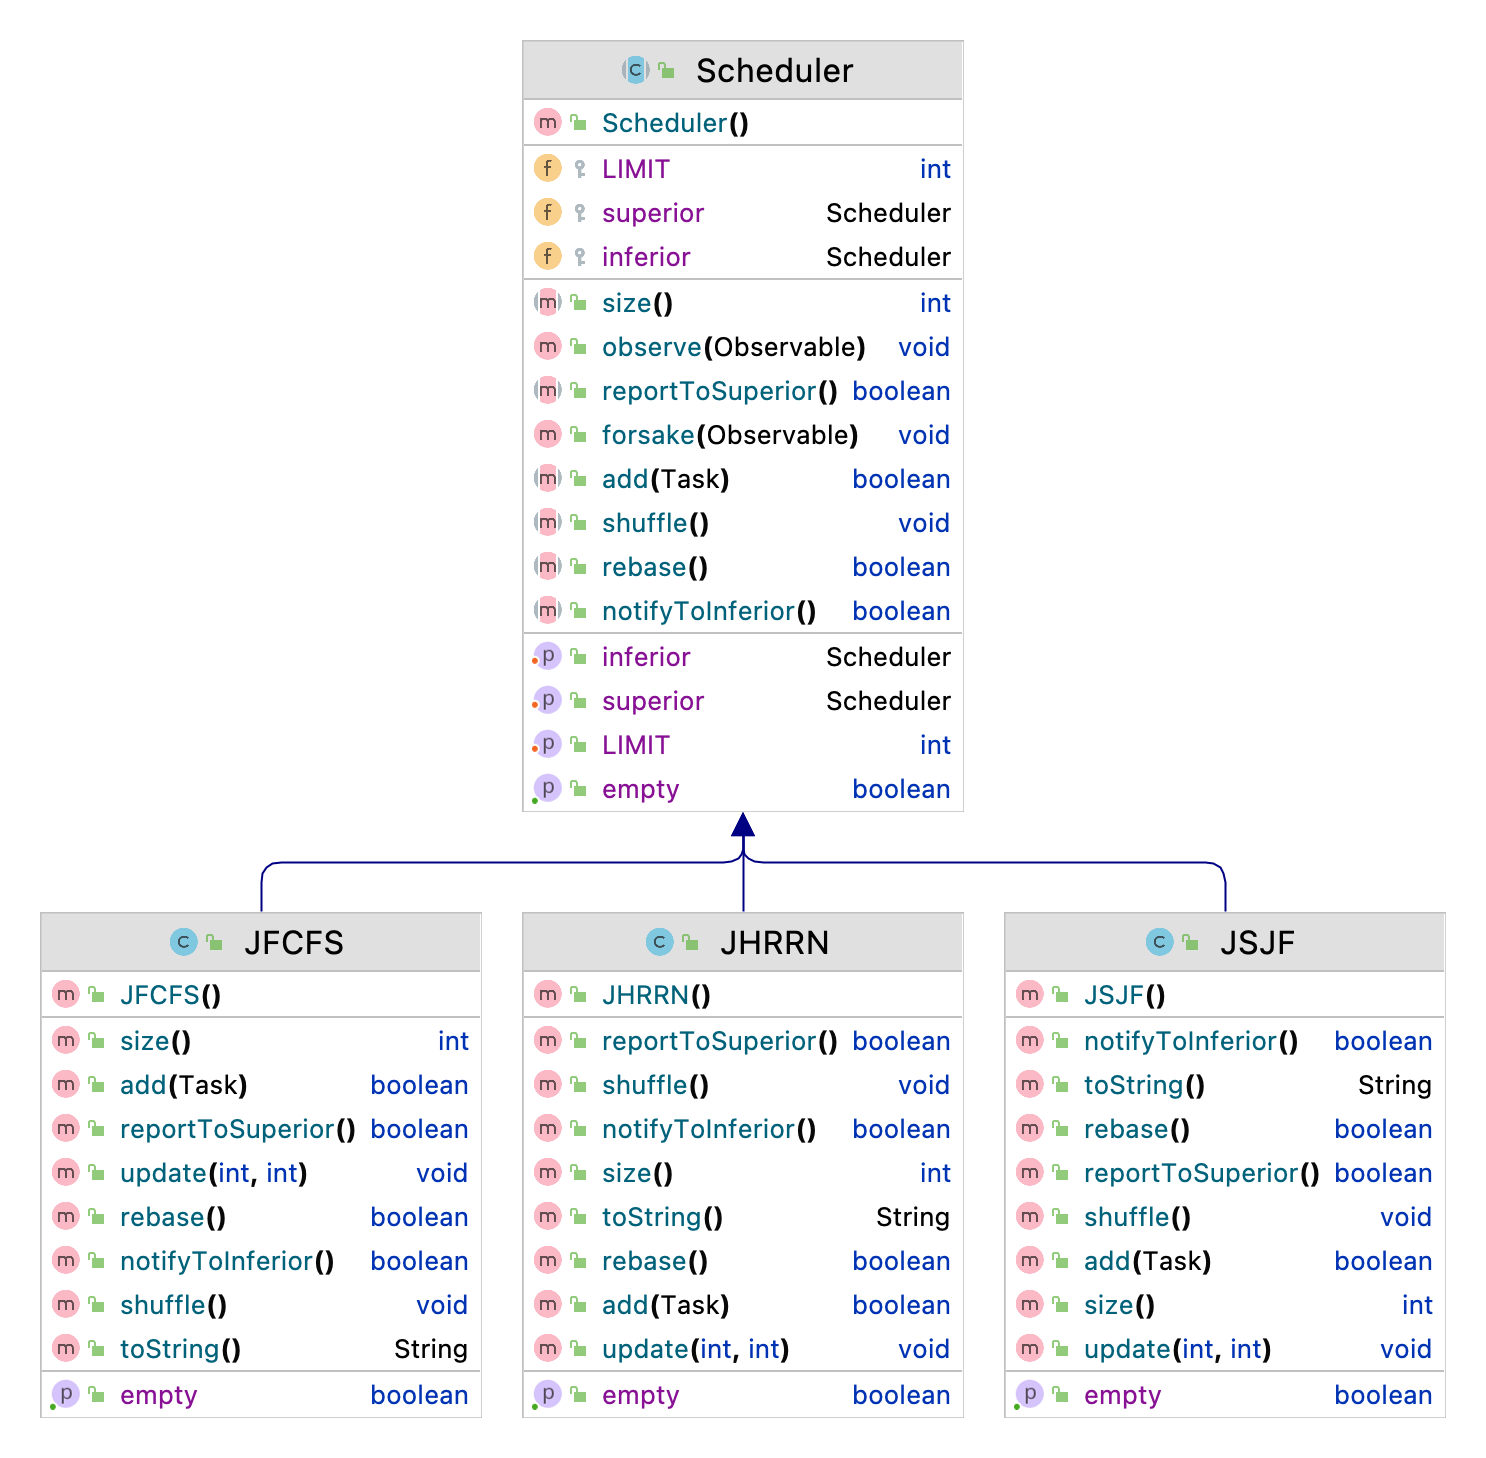
\includegraphics[height=232.5pt]{t1-class.png}
    \caption{作业调度层}
\end{figure}

作业调度的职责是按照一定的策略,向进程调度提交任务(填入内存)。FCFS、HRRN、SJF的不同主要体现于调度次序,即优先队列的比较方式。本节主要以高响应比优先实现为例,介绍抽象调度类与作业调度层。

\begin{minted}[mathescape,
    linenos,
    numbersep=5pt,
    frame=lines,
    gobble=4,
    framesep=2mm]{Java}
    public abstract class Scheduler implements Observer {
        protected int LIMIT = Integer.MAX_VALUE;
        protected Scheduler superior = null;
        protected Scheduler inferior = null;
    
        public void setLIMIT(int LIMIT) {this.LIMIT = LIMIT;}
    
        public void setSuperior(Scheduler superior) {this.superior = superior;}
    
        public void setInferior(Scheduler inferior) {this.inferior = inferior;}
    
        @Override
        public void observe(Observable target) {target.attachObserver(this);}
    
        @Override
        public void forsake(Observable target) {target.detachObserver(this);}
    
        public abstract boolean add(Task t);
    
        public abstract boolean reportToSuperior();
    
        public abstract boolean notifyToInferior();
    
        public abstract boolean rebase();
    
        public abstract int size();
    
        public abstract boolean isEmpty();
    
        public abstract void shuffle();
    }
\end{minted}

下面对于各个接口,分别解释具体实现:

\begin{lstlisting}[language={java},caption={收容队列(基于响应比的优先队列)}]
private PriorityQueue<Task> queue = new PriorityQueue<>(new Comparator<Task>() {
    @Override
    public int compare(Task o1, Task o2) {
        return (o2.getResponseRate(Clock.minutes) - o1.getResponseRate(Clock.minutes) > 0) ? (1) : (-1);
    }
});
\end{lstlisting}

\begin{lstlisting}[language={java},caption={调度方式(向上提交),调度时机(时间流逝)}]
@Override
public void update(int currentTime, int elapseUnit) {
    boolean flag = true;
    while (queue.peek() != null && flag) {
        flag = reportToSuperior();
    }
}
\end{lstlisting}

\begin{lstlisting}[language={java},caption={添加作业(收容状态)}]
@Override
public boolean add(Task t) {
    if (queue.size() >= LIMIT)
        return false;

    t.toggleBackup();
    queue.offer(t);
    return true;
}
\end{lstlisting}

\begin{lstlisting}[language={java},caption={模拟为作业创建进程,装填进入内存}]
@Override
public boolean reportToSuperior() {
    if (superior == null || queue.isEmpty())
        return false;

    shuffle();
    if (!superior.add(queue.peek()))
        return false;

    return rebase();
}
\end{lstlisting}

\begin{lstlisting}[language={java},caption={在本层队列中移除任务}]
@Override
public boolean rebase() {
    if (queue.isEmpty())
        return false;

    queue.poll();
    return true;
}
\end{lstlisting}

\begin{lstlisting}[language={java},caption={响应比动态变化,刷新队列顺序}]
@Override
public void shuffle() {
    if (queue.size() >= 2) {
        queue.offer(queue.poll());
    }
}
\end{lstlisting}

需要特别说明的是,短作业优先(SJF, Shortest Job First)也有抢占式的版本,通常被称为最短剩余时间优先。即,每当就绪队列改变时都需要进行调度,如果新到达的进程剩余时间比当前运行进程剩余时间更短,则由新进程抢占处理机,当前运行进程重新回到就绪队列。

\subsubsection{进程调度}
实现多道批处理系统(容量无限),作业调度统一使用“先来先服务”,进程调度分别使用“基于动态优先级的时间片轮转法”、“多级反馈队列法”。

\begin{figure}[htbp]
    \centering
    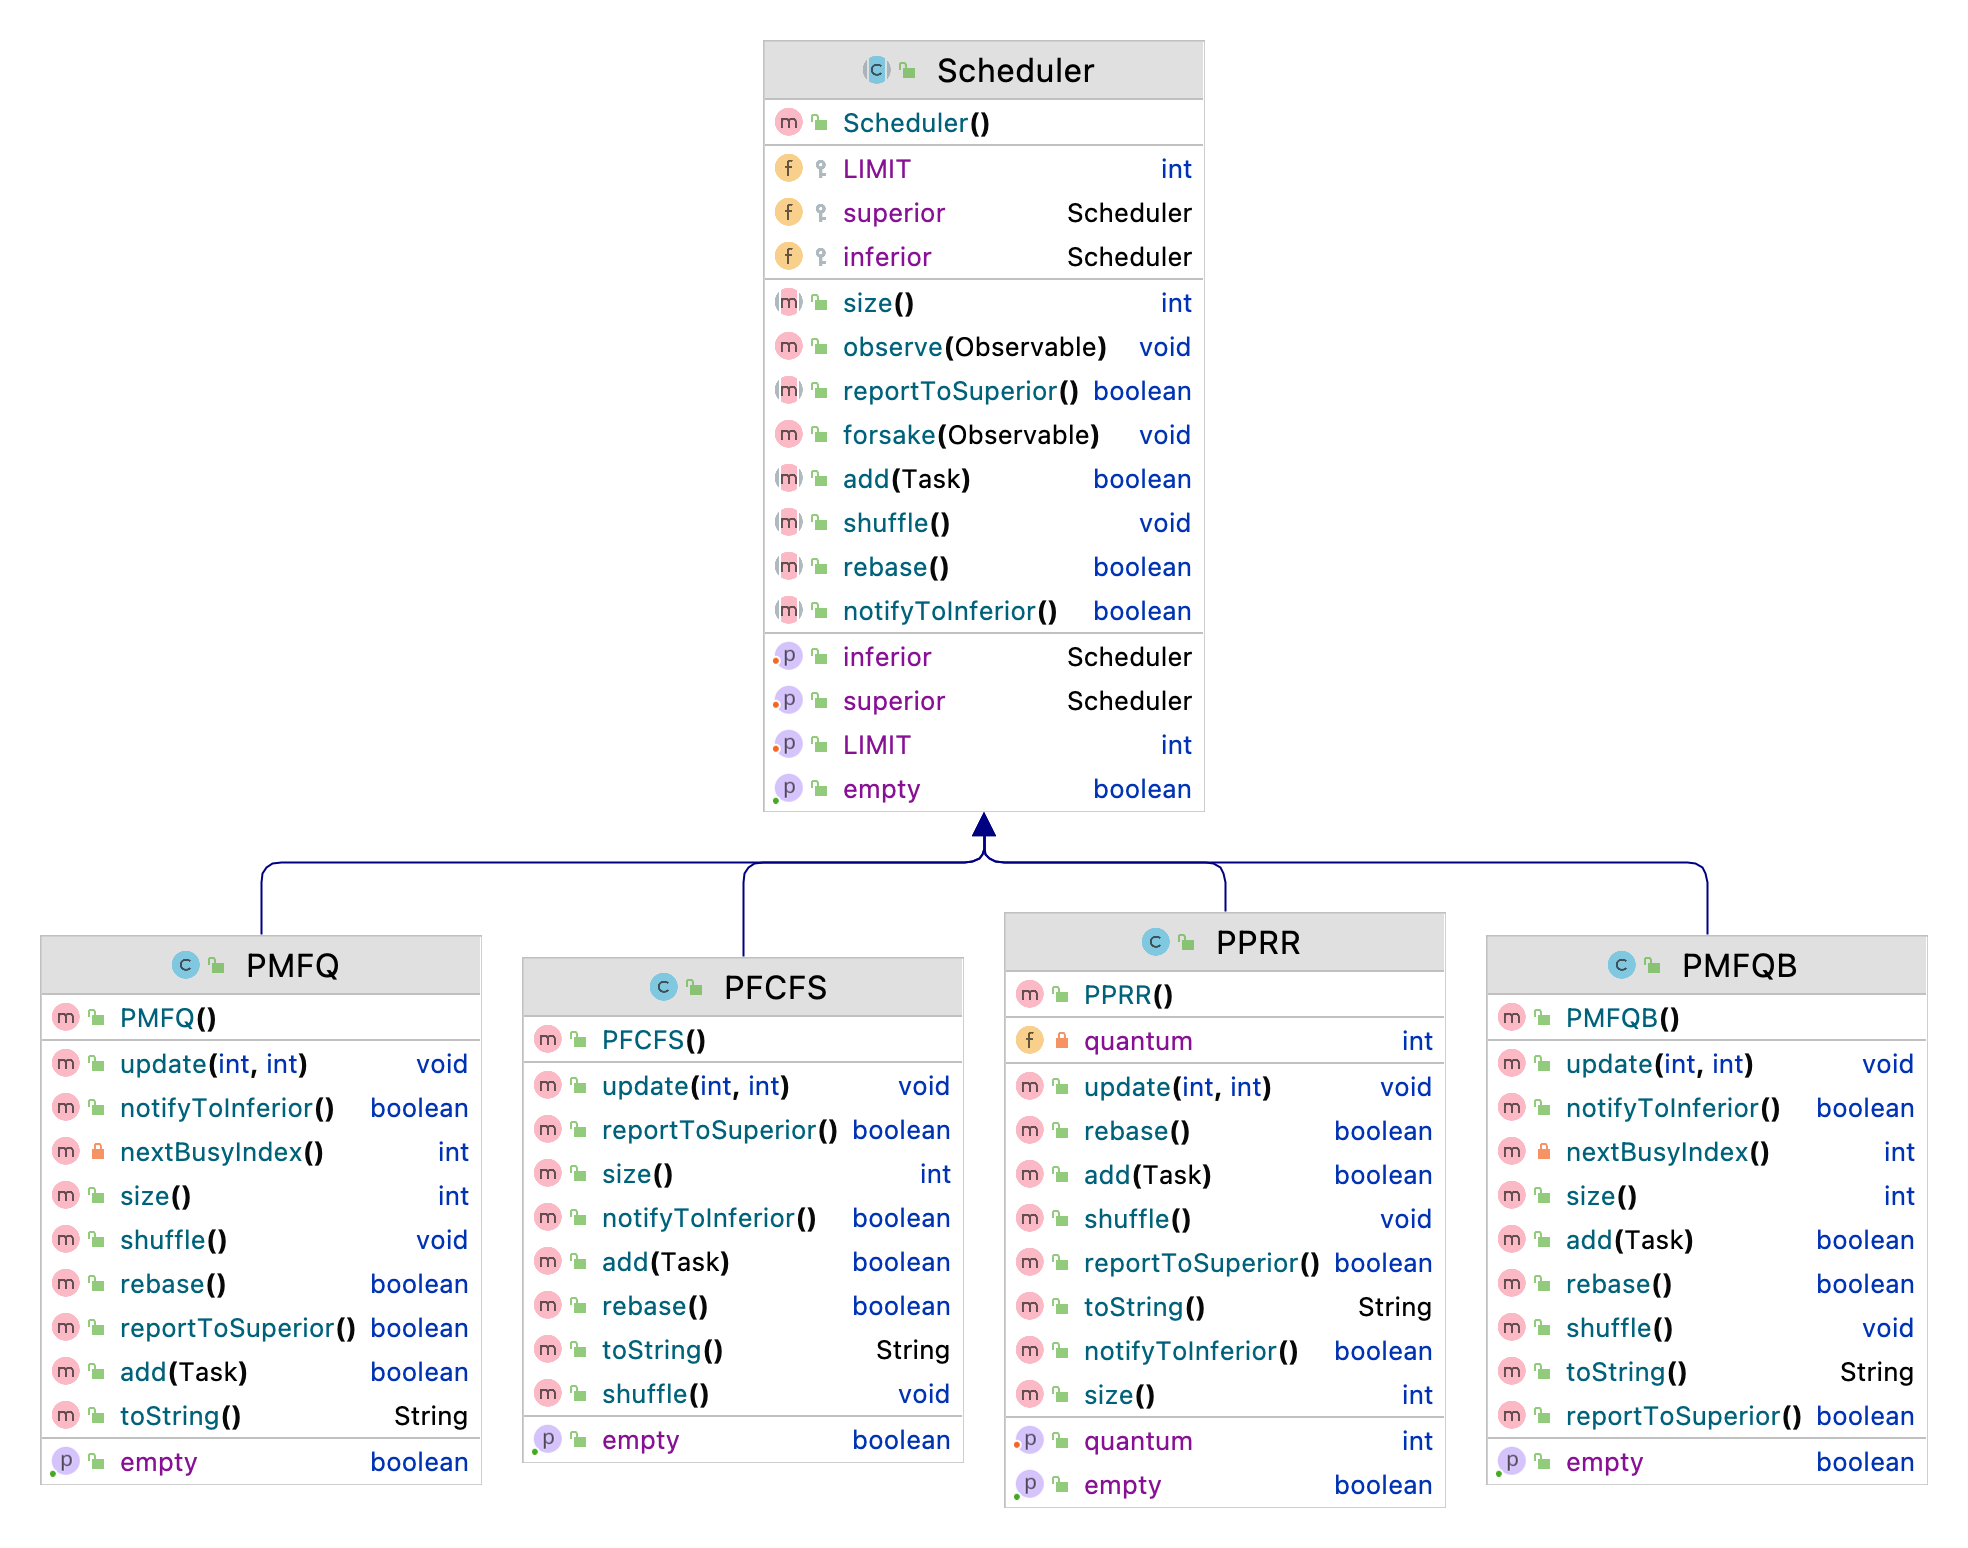
\includegraphics[scale=0.18]{t2-class.png}
    \caption{进程调度层}
\end{figure}

本节主要介绍四种算法的实现异同。共性,例如,只有进程调度会通知下层。
\begin{lstlisting}[language={java},caption={命令下层再次进行调度}]
@Override
public boolean notifyToInferior() {
    if (inferior == null)
        return false;

    return inferior.reportToSuperior();
}
\end{lstlisting}

此外,进程调度的大体框架如下:
\begin{figure}[htbp]
    \centering
    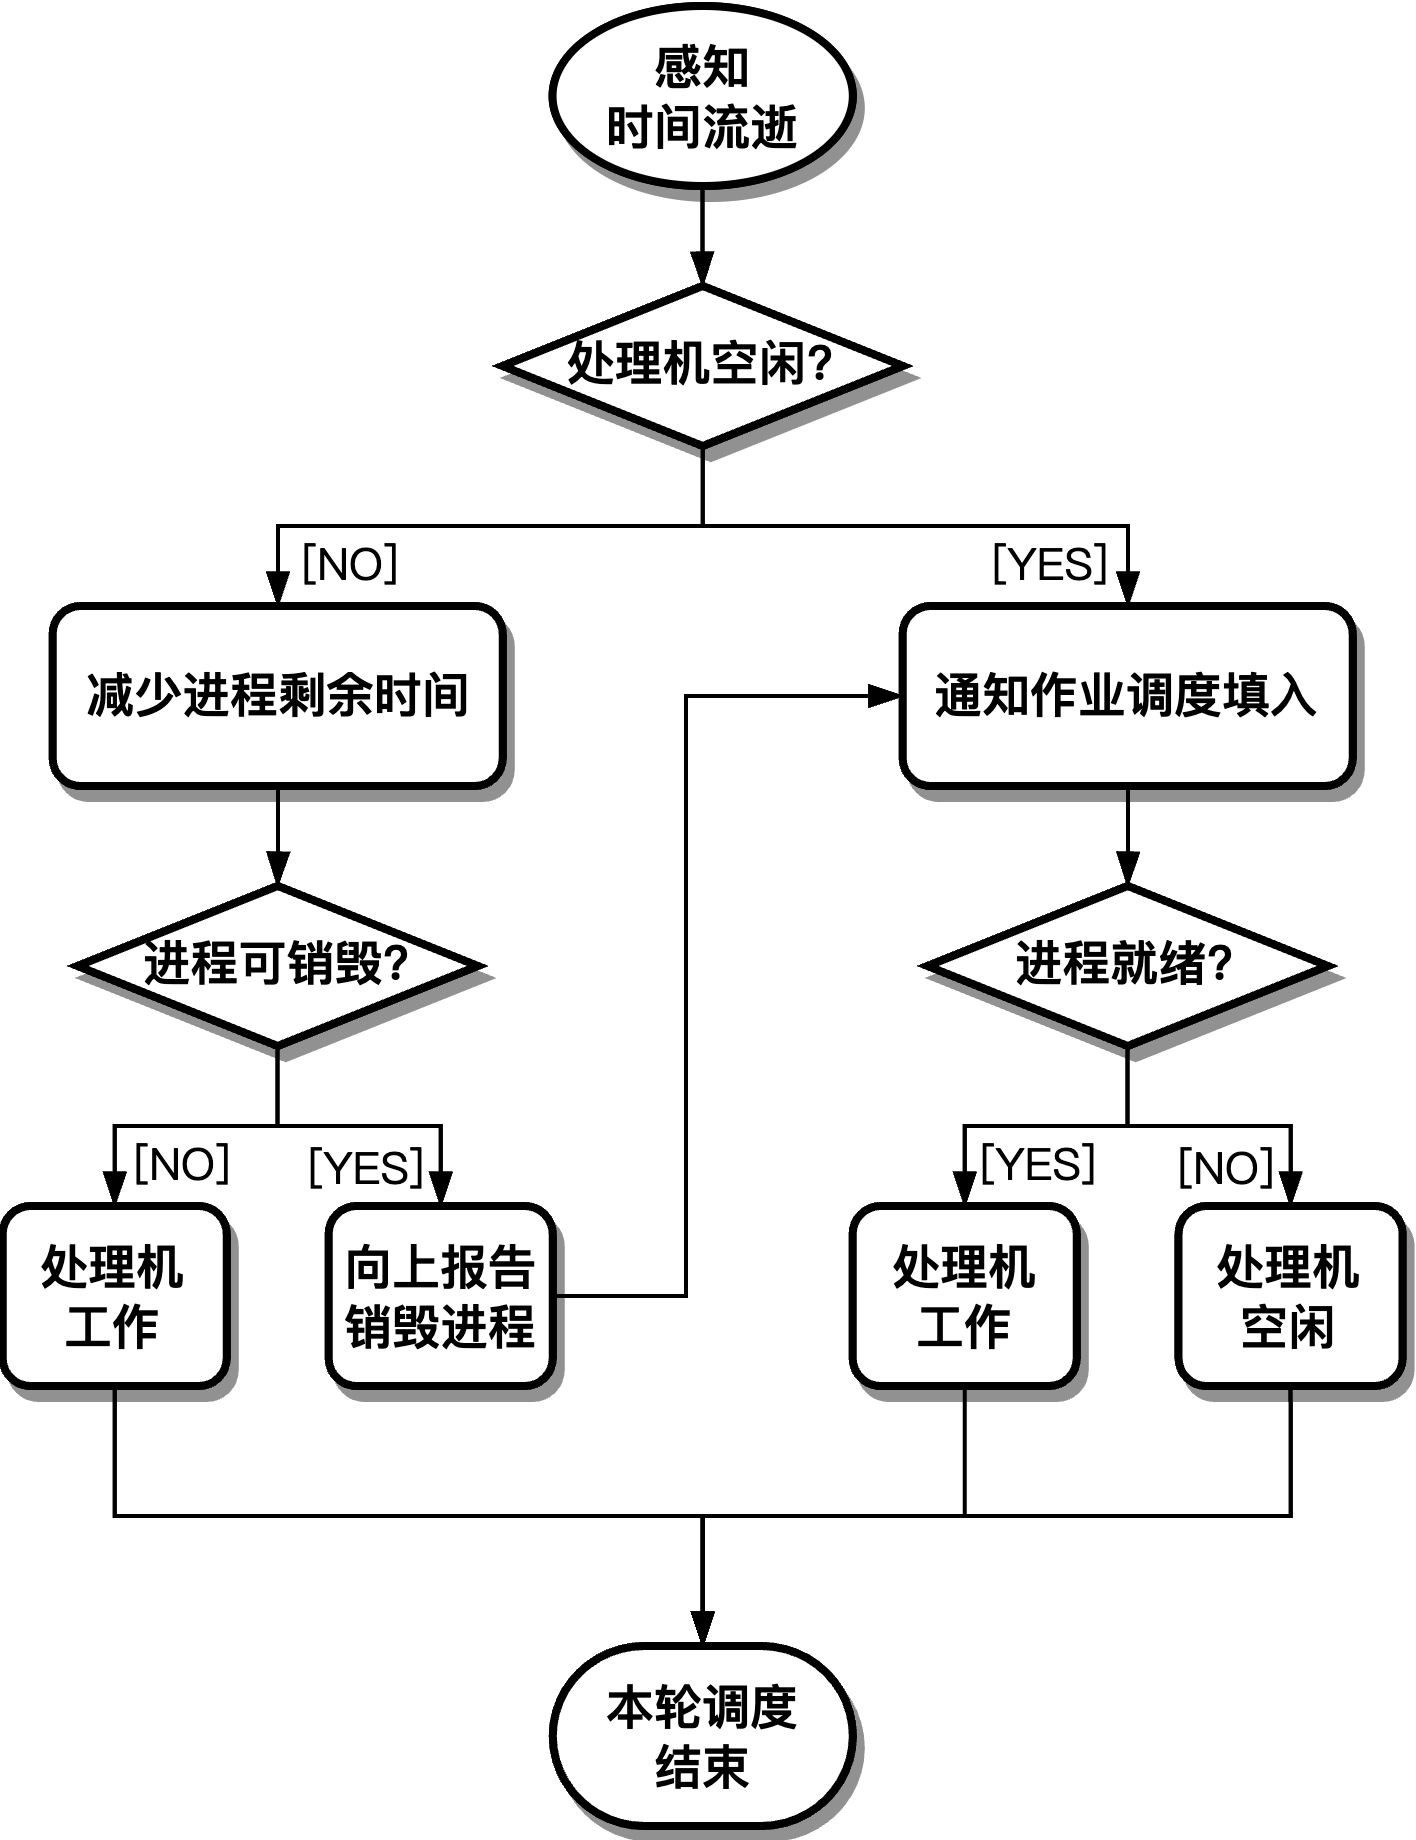
\includegraphics{i-process-fcfs.png}
    \caption{进程调度(以先来先服务为例)}
\end{figure}

不过,不同算法实现细节有所差别,下面结合代码进行分析。这里采用改进通信机制的方式避免延时问题,即,进程调度后,若向上提交销毁进程导致内存存在空余,则通知作业调度并允许其提交新的进程。

\begin{lstlisting}[language={java},caption={先来先服务}]
private boolean leisure = true;
private PriorityQueue<Task> queue = new PriorityQueue<>(Comparator.comparingInt(Task::getProcessArriveTime));

@Override
public void update(int currentTime, int elapseUnit) {
    shuffle();

    // existing a running process
    if (!leisure) {
        queue.peek().decrementLeftTime(currentTime, elapseUnit);
        if (queue.peek().isTerminated()) {
            reportToSuperior();
            leisure = true;
        } else {
            leisure = false;
        }
    }

    // needy for a ready process
    if (leisure) {
        notifyToInferior();
        if (queue.peek() != null) {
            queue.peek().toggleRunning(currentTime);
            leisure = false;
        }
    }
}
\end{lstlisting}

基于动态优先级的时间片轮转要求对时间片动态判定修改。此外,程序没有记录运行进程的引用,所以必须通过tricks保证运行进程优先级永远最高。

\begin{lstlisting}[language={java},caption={Getter(以优先级为例)}]
public int getPriority() {
    int factor = (isRunning()) ? (-1) : (1);
    return priority * factor;
}
\end{lstlisting}

\begin{lstlisting}[language={java},caption={基于动态优先级的时间片轮转}]
private boolean leisure = true;
private int quantum = 2;
private int dynamicTimeSlice = quantum;
private PriorityQueue<Task> queue = new PriorityQueue<>(new Comparator<Task>() {
    @Override
    public int compare(Task o1, Task o2) {
        return (o1.getPriority() - o2.getPriority() != 0) ? (o1.getPriority() - o2.getPriority()) : (o1.getJobSubmitTime() - o2.getJobSubmitTime());
        // return o1.getPriority() - o2.getPriority();
    }
});

public void setQuantum(int quantum) {
    this.quantum = quantum;
}

public void update(int currentTime, int elapseUnit) {
    shuffle();

    // existing a running process within the last minute
    if (!leisure) {
        queue.peek().decrementLeftTime(currentTime, elapseUnit);
        dynamicTimeSlice -= elapseUnit;
        // terminated
        if (queue.peek().isTerminated()) {
            queue.peek().incrementPriority(2);
            reportToSuperior();
            // reset time slice
            leisure = true;
        } else if (queue.peek().isRunning()) {
            // brute-force offline
            if (dynamicTimeSlice == 0) {
                queue.peek().incrementPriority(2);
                queue.peek().toggleReReady();
                shuffle();
                leisure = true;
            }
            // slice is still adequate for continuous running
            else {
                leisure = false;
            }
        }
    }

    // needy for a ready process
    if (leisure) {
        dynamicTimeSlice = quantum;
        notifyToInferior();
        if (queue.peek() != null) {
            queue.peek().toggleRunning(currentTime);
            leisure = false;
        }
    }

}
\end{lstlisting}

多级反馈队列法:设置多级就绪队列,各级队列优先级从高到低,时间片由小到大。新进程到达时,先进入第一级队列,按“先来先服务”原则排队等待。若时间片用完进程仍未结束,则将该进程移入下级队列队尾(直到最后一级)。只有第$k$级队列为空,才会为$k+1$级队头进程分配时间片。

\begin{lstlisting}[language={java},caption={多级反馈队列(数据结构)}]
private List<Deque<Task>> queues = new ArrayList<>();
private boolean leisure = true;
private int busyIndex = 0;
private int quantum = 1;
private int dynamicTimeSlice = quantum;

public PMFQ() {
    Deque<Task> top = new ArrayDeque<>();
    queues.add(top);
    Deque<Task> mid = new ArrayDeque<>();
    queues.add(mid);
    Deque<Task> btm = new ArrayDeque<>();
    queues.add(btm);
\end{lstlisting}

多级反馈队列法同样可分为抢占式和非抢占式,这两种实现的主要区别在于“调度时机”。假设当前运行进程优先级并非顺位第一,即使时间片未运行完,抢占式调度也会收回剩余时间片使优先级更高的新进程获得处理机资源,并将被抢占处理机的进程重新放回原队列队尾。而非抢占式调度须要等时间片轮转才可以调度。
\begin{lstlisting}[language={java},caption={多级反馈队列(非抢占式调度)}]
@Override
public void update(int currentTime, int elapseUnit) {
    // existing a running process within the last minute
    if (!leisure) {
        Deque<Task> queue = queues.get(busyIndex);
        queue.peek().decrementLeftTime(currentTime, elapseUnit);
        dynamicTimeSlice -= elapseUnit;
        // terminated
        if (queue.peek().isTerminated()) {
            reportToSuperior();
            // reset time slice
            leisure = true;
        } else if (queue.peek().isRunning()) {
            // brute-force offline
            if (dynamicTimeSlice == 0) {
                queue.peek().toggleReReady();
                int nextIndex = Math.min(busyIndex + 1, 2);
                // next level or bottom
                queues.get(nextIndex).offer(queue.poll());
                leisure = true;
            }
            // slice is still adequate for continuous running
            else {
                leisure = false;
            }
        }
    }

    // needy for a ready process
    if (leisure) {
        notifyToInferior();
        // somebody ready
        if (nextBusyIndex() != -1) {
            busyIndex = nextBusyIndex();
            quantum = (int) Math.pow(2, busyIndex);
            dynamicTimeSlice = quantum;

            Deque<Task> queue = queues.get(busyIndex);
            queue.peek().toggleRunning(currentTime);
            leisure = false;
        }
    }
}
\end{lstlisting}

\begin{lstlisting}[language={java},caption={多级反馈队列(抢占式调度)}]
@Override
public void update(int currentTime, int elapseUnit) {
    // existing a running process within the last minute
    if (!leisure) {
        Deque<Task> queue = queues.get(busyIndex);
        queue.peek().decrementLeftTime(currentTime, elapseUnit);
        dynamicTimeSlice -= elapseUnit;
        // terminated
        if (queue.peek().isTerminated()) {
            reportToSuperior();
            // reset time slice
            leisure = true;
        } else if (queue.peek().isRunning()) {
            // brute-force offline
            if (dynamicTimeSlice == 0) {
                queue.peek().toggleReReady();
                int nextIndex = Math.min(busyIndex + 1, 2);
                // next level or bottom
                queues.get(nextIndex).offer(queue.poll());
                leisure = true;
            }
            // slice is still adequate for continuous running
            else {
                // nobody can forcibly occupy
                if (nextBusyIndex() == busyIndex) {
                    leisure = false;
                } else {
                    // FIXME
                    queue.peek().toggleReReady();
                    queue.offer(queue.poll());
                    leisure = true;
                }
            }
        }
    }

    // needy for a ready process
    if (leisure) {
        notifyToInferior();
        // somebody ready
        if (nextBusyIndex() != -1) {
            busyIndex = nextBusyIndex();
            quantum = (int) Math.pow(2, busyIndex);
            dynamicTimeSlice = quantum;

            Deque<Task> queue = queues.get(busyIndex);
            queue.peek().toggleRunning(currentTime);
            leisure = false;
        }
    }
}
\end{lstlisting}

\subsection{边缘实现}

选择使用Android移动平台部署应用,以省去云服务器环境搭建。

\subsubsection{依赖配置}

\begin{minted}{groovy}
android {
    namespace 'edu.wust.durui'
    compileSdk 32
    defaultConfig {
        vectorDrawables.useSupportLibrary = true
        multiDexEnabled true
        applicationId "edu.wust.durui"
        minSdk 29
        targetSdk 32
        versionCode 1
        versionName "1.0"
        ...
    }
    ...
    viewBinding {
        enabled = true
    }
    dataBinding {
        enabled = true
    }
}
dependencies {
    ...
    implementation 'com.google.android.material:material:1.6.1'
    implementation "androidx.lifecycle:lifecycle-livedata-ktx:2.4.1"
    implementation "androidx.lifecycle:lifecycle-viewmodel-ktx:2.5.1"
    implementation "androidx.multidex:multidex:2.0.1"
    implementation "androidx.fragment:fragment:1.5.5"
    implementation 'com.github.blackfizz:eazegraph:1.2.2@aar'
    implementation 'com.nineoldandroids:library:2.4.0'
    implementation 'com.github.vipulasri:timelineview:1.1.5'
}
\end{minted}

\subsubsection{核心技术}

\begin{description}
    \item[MVVM]
        应用架构定义了应用的各个部分之间的界限以及每个部分应承担的职责,遵循“关注点分离”、“数据驱动界面”、“单一数据源和单向数据流”,避免在Activity或Fragment编写所有代码。
    \item[Fragment]
        Fragment组件介于Activity和View:一方面,它未继承Context,无法独立存在,必须作为宿主视图的一部分;可另一方面,它又可以定义管理自己的布局,具有自己的生命周期(Lifecycle)。
    \item[ViewModel]
        配置更改(例如旋转屏幕)时,UI数据可能丢失,是因为界面被系统自动销毁重绘(和会输销毁整个程序不同),同时,界面类的成员变量也被回收。一个解决方案是,将数据的所有权和界面交互逻辑分离开;如此,系统只回收Activity类中的对数据类的“引用”,并不会影响数据类本身。

        当ViewModel中存在一个LiveData容器,可以指定当前数据的观察者(Observer),即每当LiveData中存放的数据发生变化时,观察者可以全自动地执行操作,例如,改变UI界面中的数据。相比起定时检测更新和通知模式,观察者具有强大生命力和无比优越性。
    \item[RecyclerView] 核心视图组件之一。RecyclerView可以轻松高效地显示大量数据,当提供数据并定义每个列表项的外观后,RecyclerView
        库会根据需要动态创建元素。
    \item[DatePicker]
        核心视图组件之一。DatePicker继承自FrameLayout类,日期选择控件的主要功能是向用户提供包含年、月、日的日期数据并允许用户对其修改。如果要捕获用户修改日期选择控件中的数据事件,需要为DatePicker添加OnDateChangedListener监听器。
    \item[EazeGraph]
        核心视图组件之一。轻量级的图表库\footnote{https://github.com/paulroehr/EazeGraph},支持生成四种图表:条形图,层叠柱状图,饼状图,折线图。
    \item[TimelineView]
        核心视图组件之一。轻量级时间视图库\footnote{https://github.com/vipulasri/Timeline-View},支持呈现时间线,应用广泛,如物流追踪历史节点等。

\end{description}

\subsection{界面设计}

\begin{figure}[htbp]
    \centering
    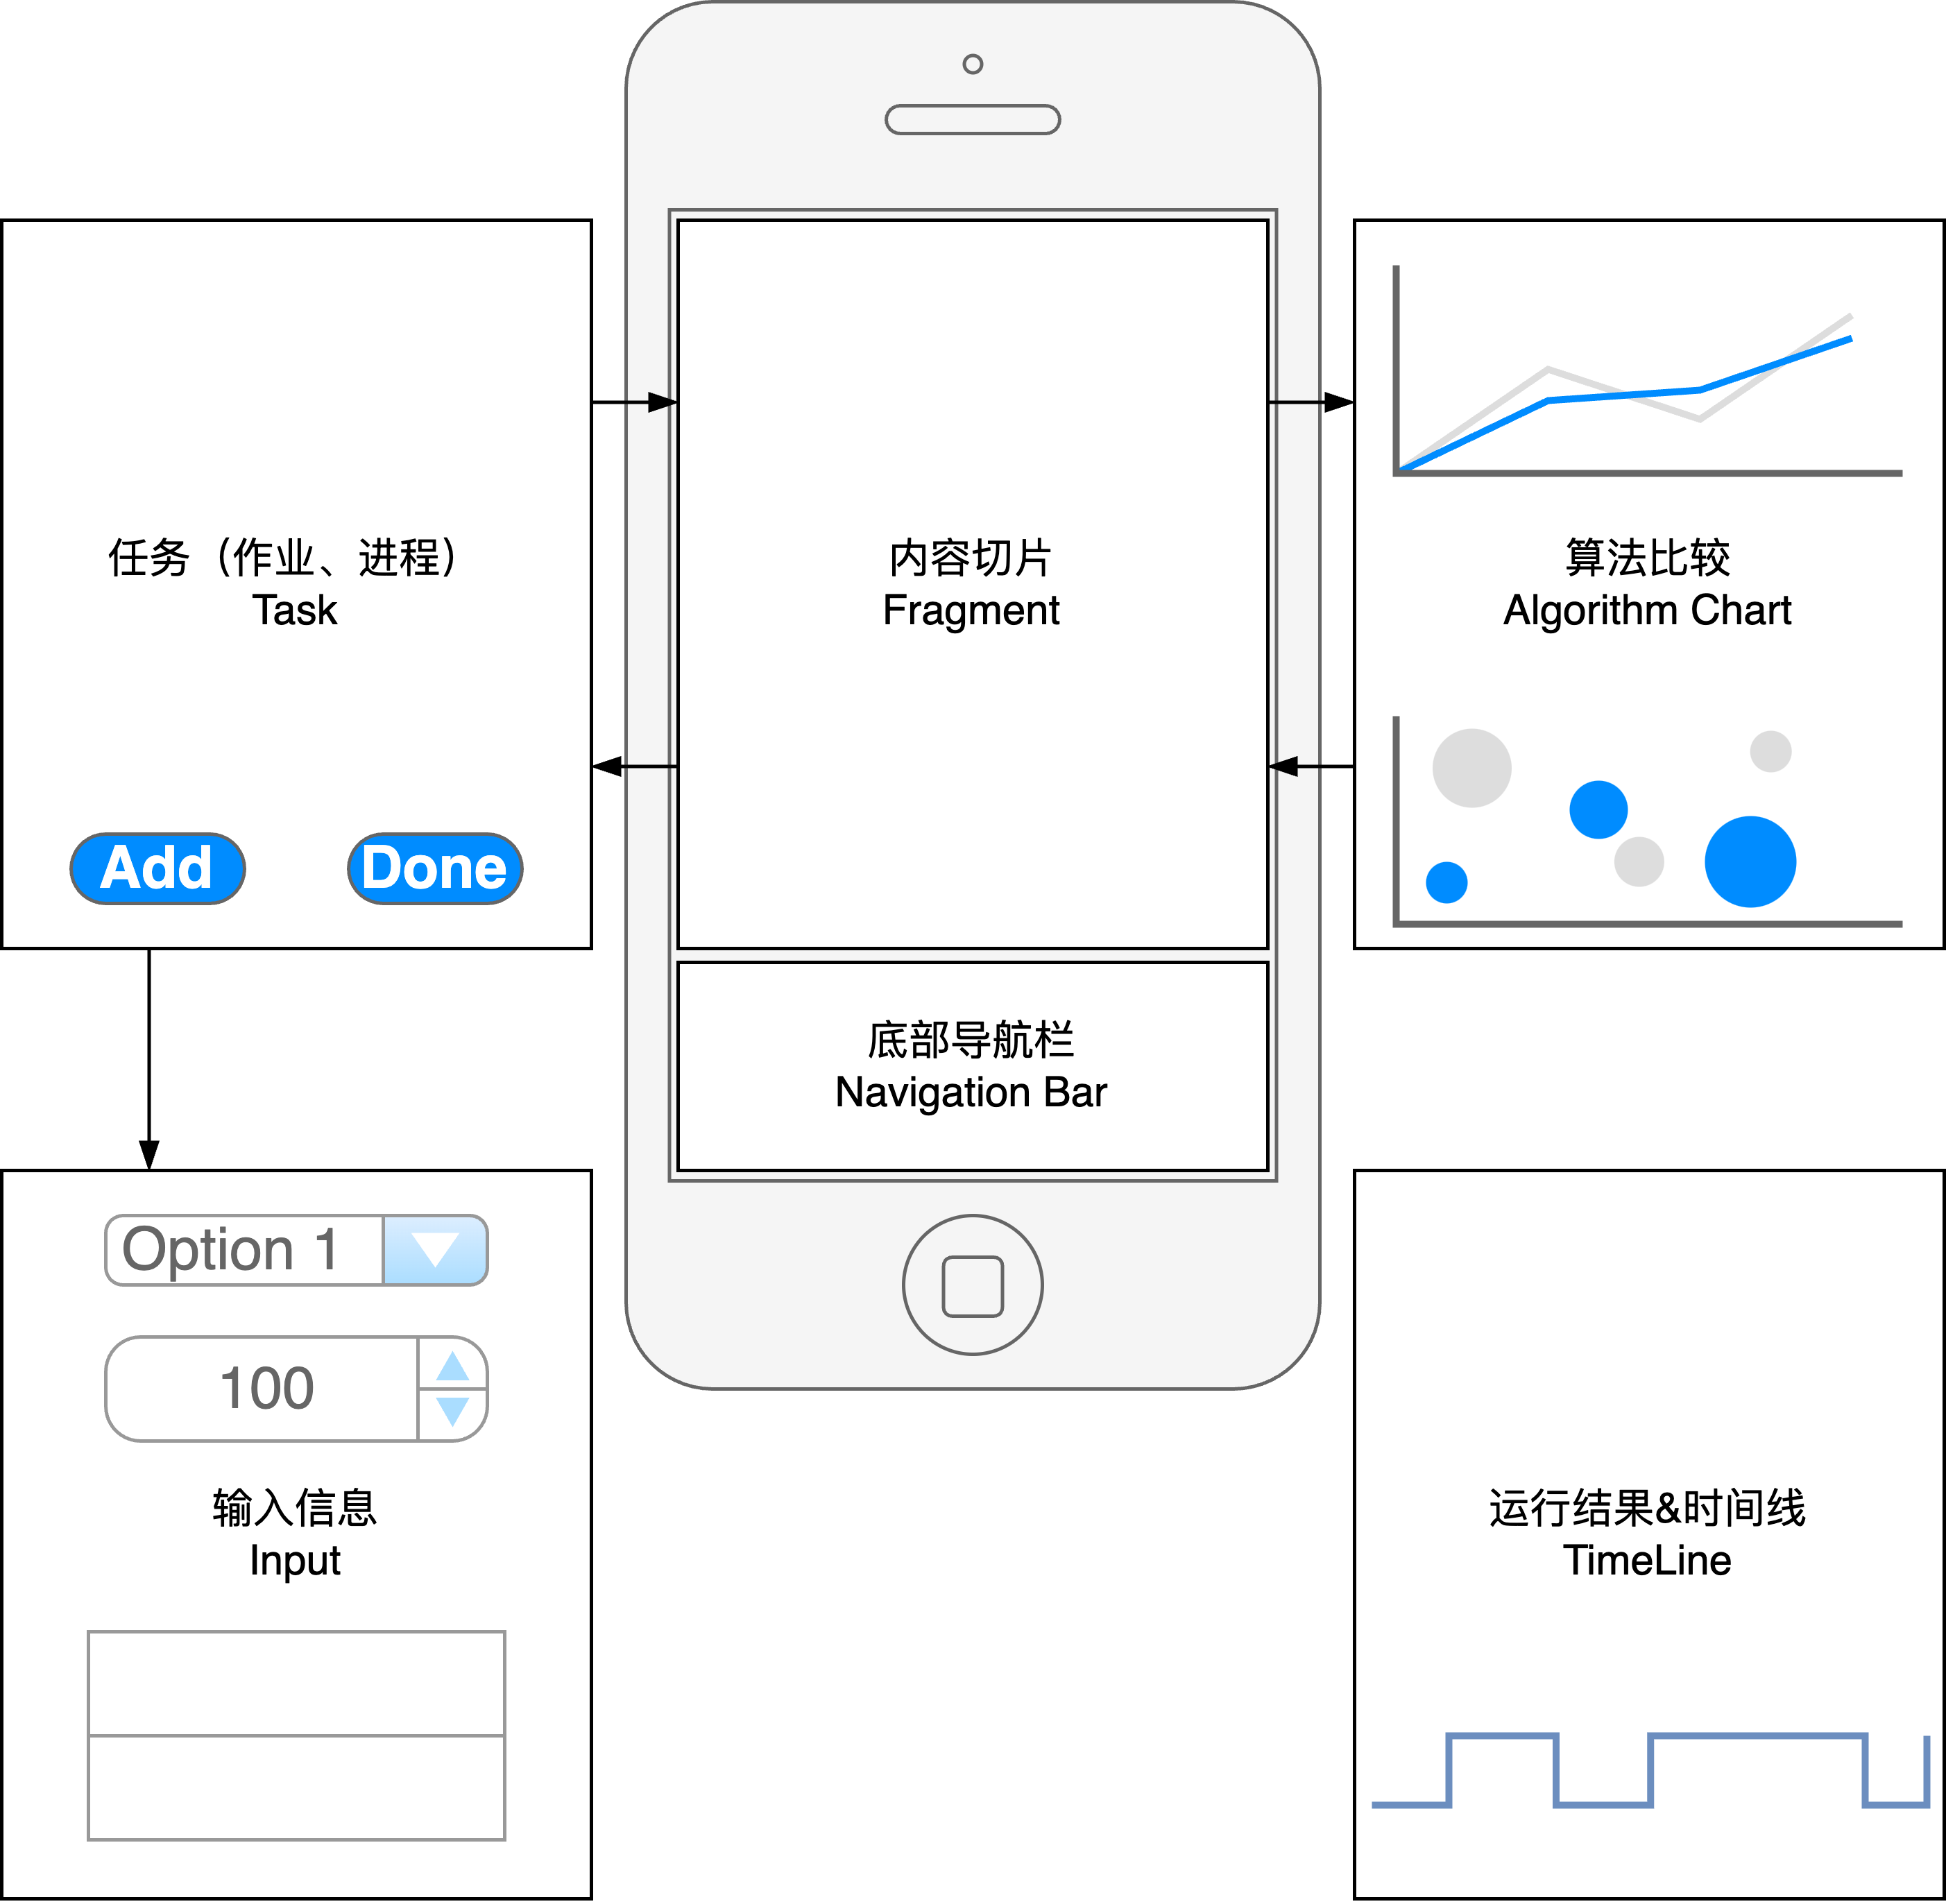
\includegraphics[scale=0.09]{i-prototype.png}
    \caption{界面原型设计图}
\end{figure}

\section{系统测试}

\subsection{测试用例}

\begin{table}[htbp]
    \caption{测试用例(先来先服务,平均周转时间1.725h)}
    \centering
    \begin{tabular}{cccccc}
        \toprule
        作业 & 进入时刻 & 运行时间(分钟) & 开始时刻 & 完成时刻 & 周转时间(分钟) \\
        \midrule
        1    & 08:00    & 120              & 08:00    & 10:00    & 120              \\
        2    & 08:30    & 30               & 10:00    & 10:30    & 120              \\
        3    & 09:00    & 6                & 10:30    & 10:36    & 96               \\
        4    & 09:30    & 12               & 10:36    & 10:48    & 78               \\
        \bottomrule
    \end{tabular}
    \qquad
\end{table}

\begin{table}[htbp]
    \caption{测试用例(短作业优先,平均周转时间1.550h)}
    \centering
    \begin{tabular}{cccccc}
        \toprule
        作业 & 进入时刻 & 运行时间(小时) & 开始时刻 & 完成时刻 & 周转时间(小时) \\
        \midrule
        1    & 08:00    & 2.00             & 08:00    & 10:00    & 2.00             \\
        2    & 08:30    & 0.50             & 10:18    & 10:48    & 2.30             \\
        3    & 09:00    & 0.10             & 10:00    & 10:06    & 1.10             \\
        4    & 09:30    & 0.20             & 10:06    & 10:18    & 0.80             \\
        \bottomrule
    \end{tabular}
    \qquad
\end{table}

\begin{table}[htbp]
    \caption{测试用例(高响应比优先,平均周转时间1.625h)}
    \centering
    \begin{tabular}{cccccc}
        \toprule
        作业 & 进入时刻 & 运行时间(小时) & 开始时刻 & 完成时刻 & 周转时间(小时) \\
        \midrule
        1    & 08:00    & 2.00             & 08:00    & 10:00    & 2.00             \\
        2    & 08:30    & 0.50             & 10:06    & 10:36    & 2.10             \\
        3    & 09:00    & 0.10             & 10:00    & 10:06    & 1.10             \\
        4    & 09:30    & 0.20             & 10:36    & 10:48    & 1.30             \\
        \bottomrule
    \end{tabular}
    \qquad
\end{table}

\begin{table}[htbp]
    \caption{测试用例(248抢占式多级反馈队列)}
    \centering
    \begin{tabular}{cccccc}
        \toprule
        作业 & 进入时刻 & 服务时间 & 完成时刻 & 周转时间 \\
        \midrule
        A    & 0        & 7        & 11       & 11       \\
        B    & 5        & 4        & 19       & 14       \\
        C    & 7        & 13       & 30       & 23       \\
        D    & 12       & 9        & 33       & 21       \\
        \bottomrule
    \end{tabular}
    \qquad
\end{table}

\begin{table}[htbp]
    \caption{测试用例(124非抢占式多级反馈队列)}
    \centering
    \begin{tabular}{cccccc}
        \toprule
        作业 & 进入时刻 & 服务时间 & 完成时刻 & 周转时间 \\
        \midrule
        A    & 0        & 3        & 3        & 3        \\
        B    & 2        & 6        & 17       & 15       \\
        C    & 4        & 3        & 18       & 14       \\
        D    & 6        & 5        & 20       & 14       \\
        E    & 8        & 2        & 14       & 6        \\
        \bottomrule
    \end{tabular}
    \qquad
\end{table}

\subsection{运行结果}

见尾页。

\begin{figure}[h]
    \centering
    \subfigure[任务列表]{
        \begin{minipage}[t]{0.42\linewidth}
            \centering
            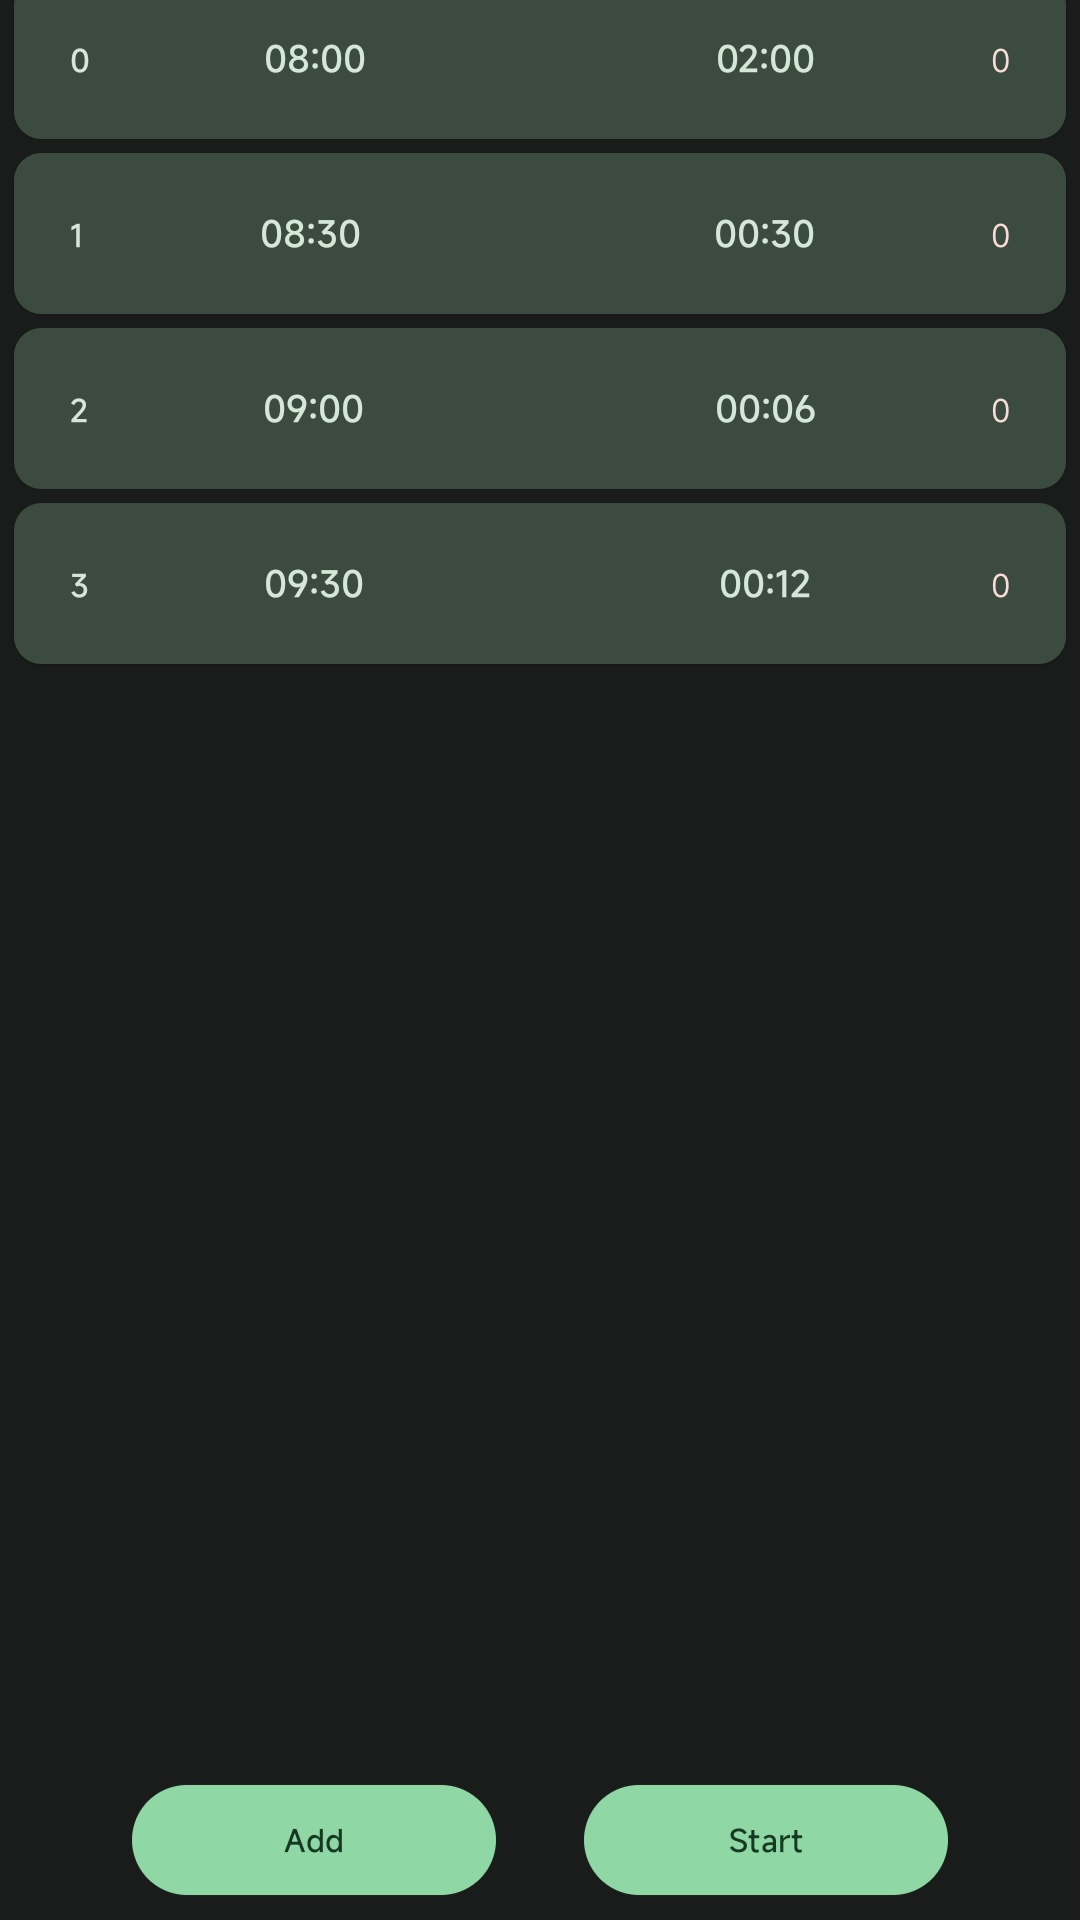
\includegraphics[width=2in]{app-list.jpg}
        \end{minipage}
    }
    \subfigure[时刻输入]{
        \begin{minipage}[t]{0.42\linewidth}
            \centering
            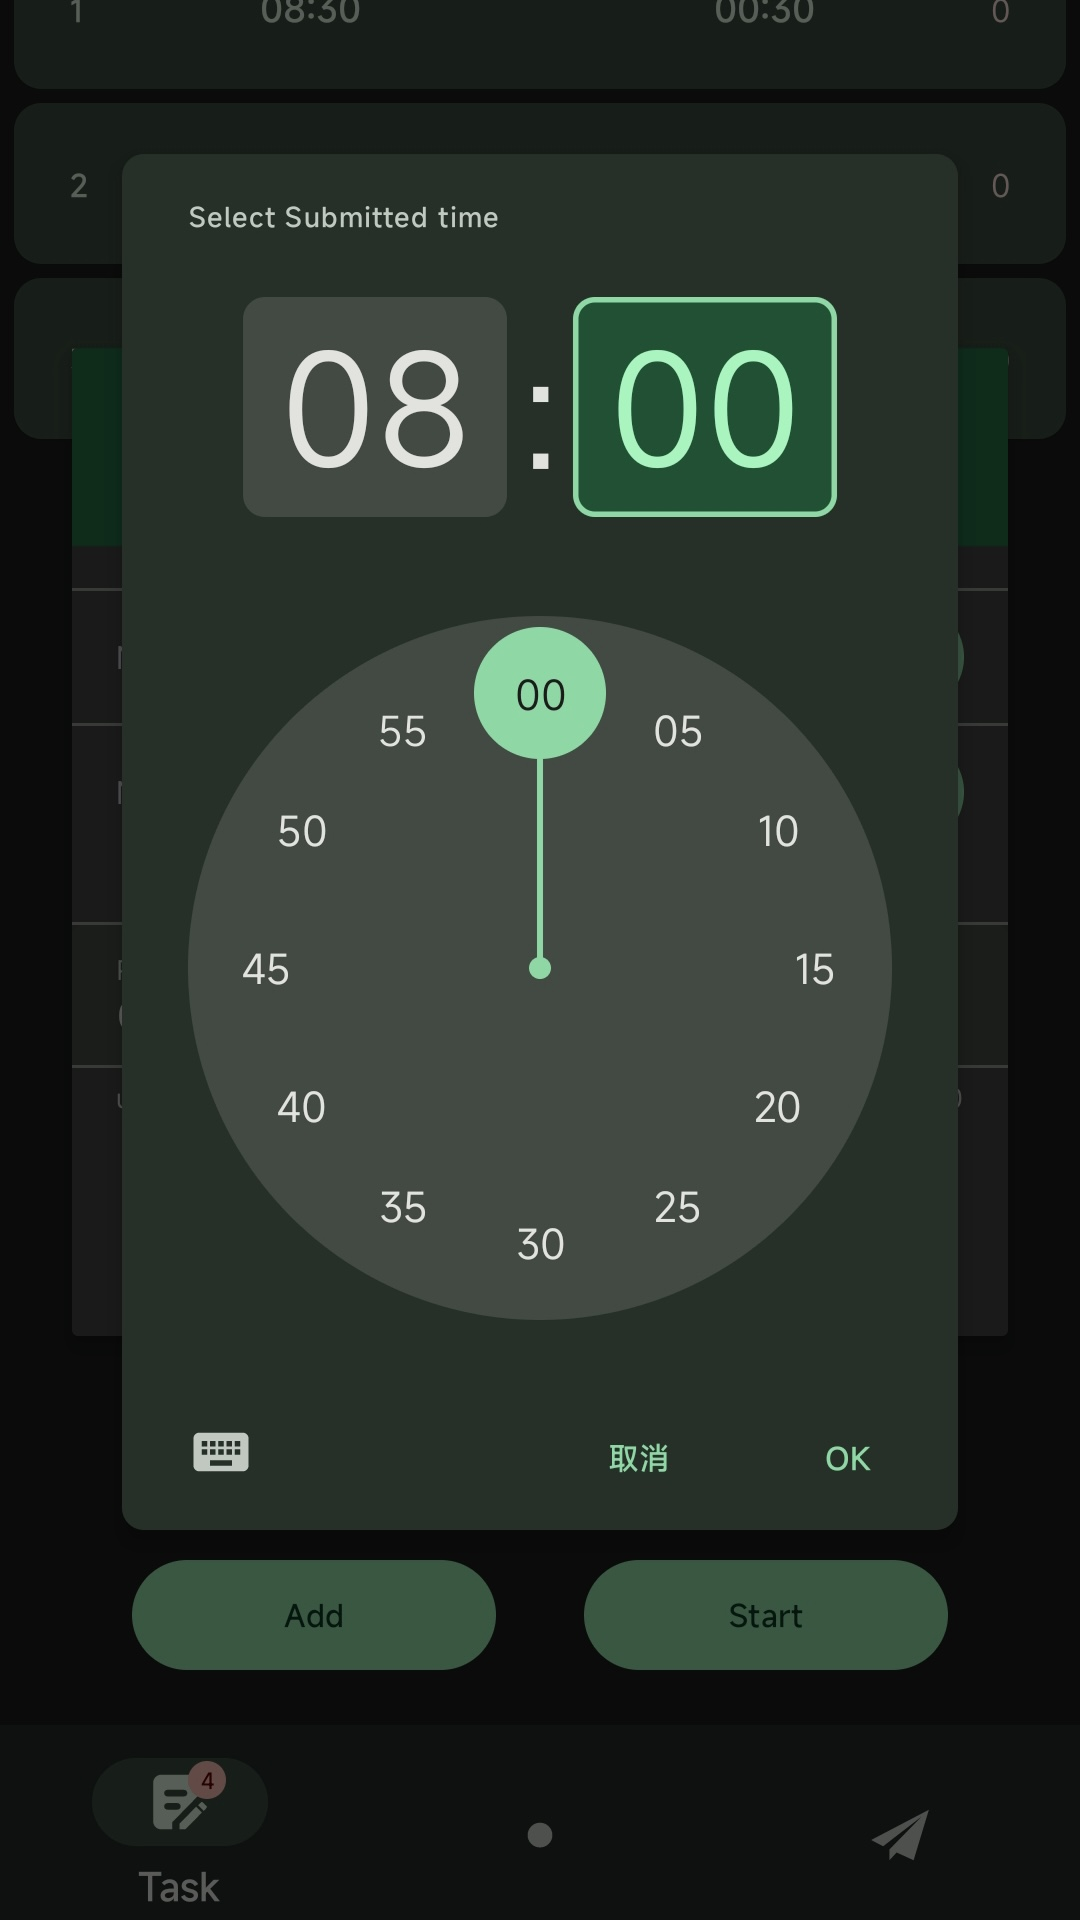
\includegraphics[width=2in]{app-clock.jpg}
        \end{minipage}%
    }
    \quad

    \subfigure[性能比较]{
        \begin{minipage}[t]{0.42\linewidth}
            \centering
            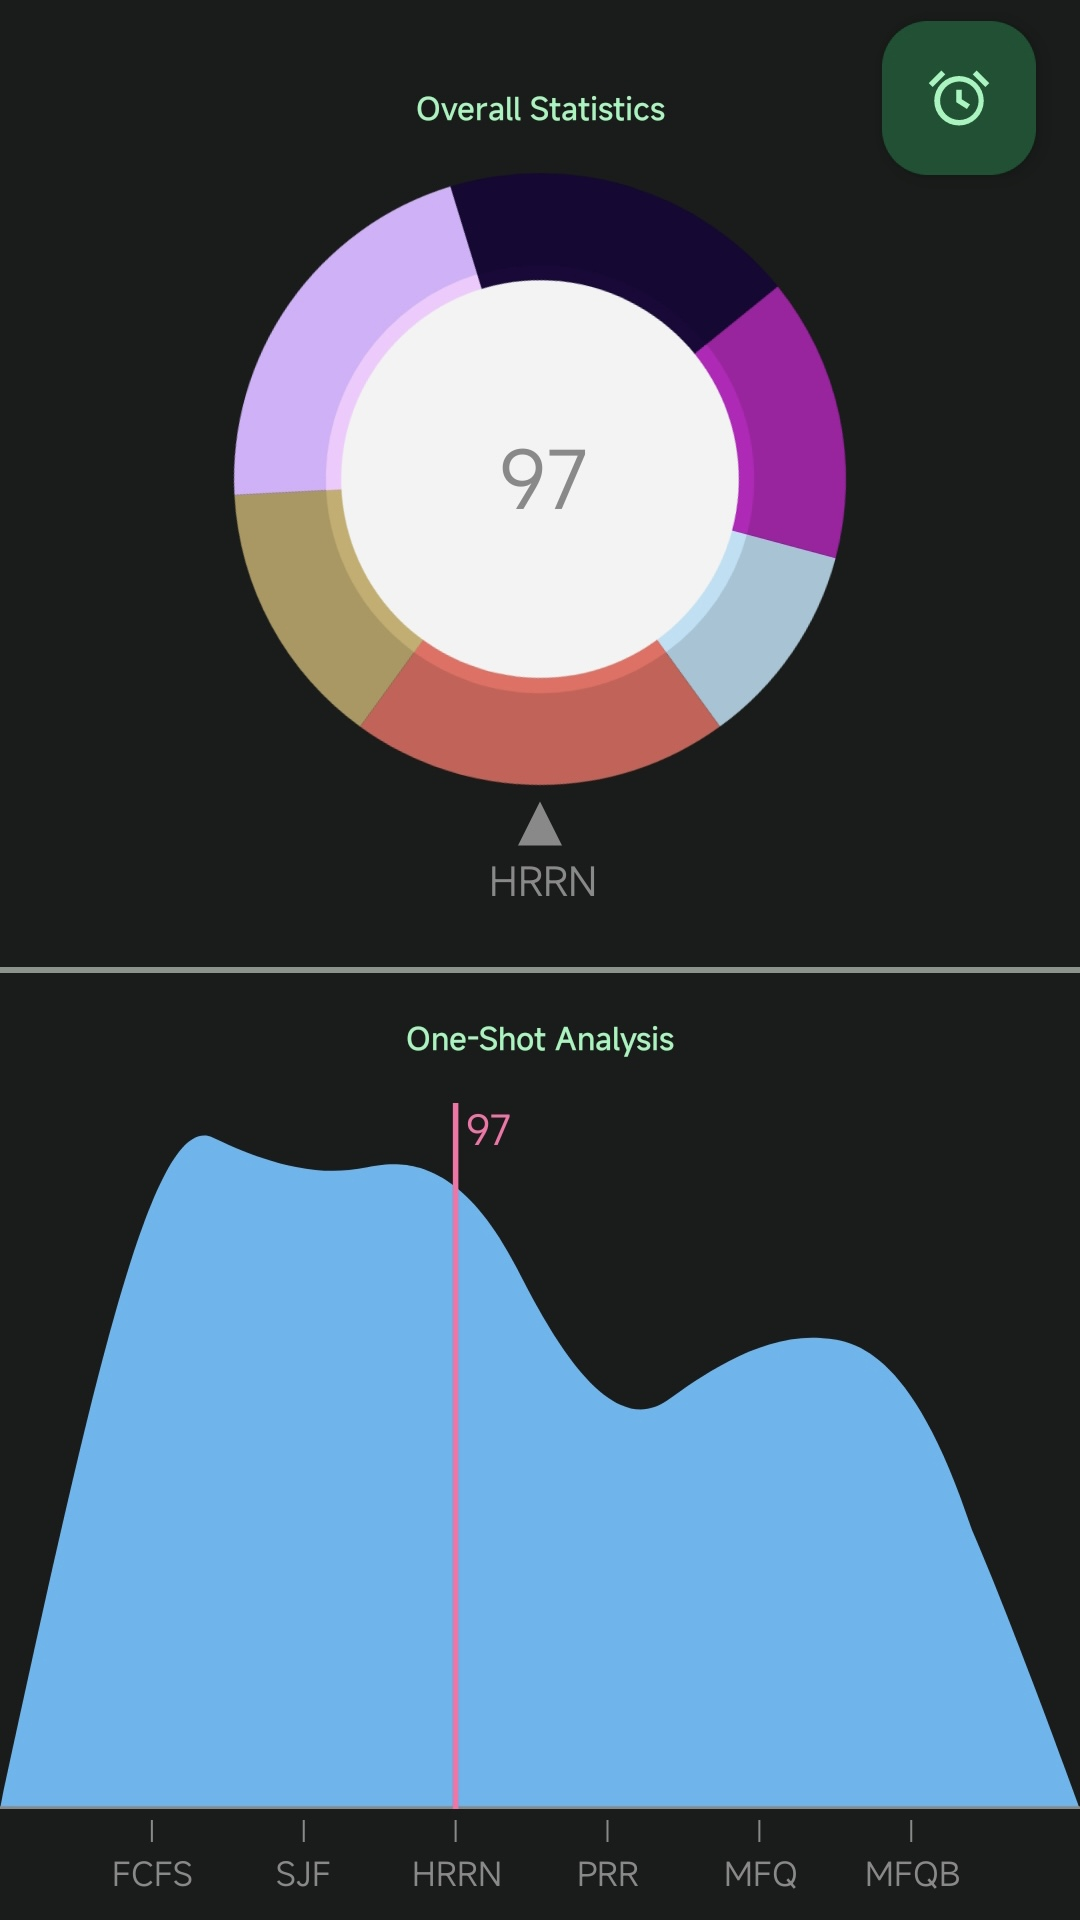
\includegraphics[width=2in]{app-statistics.jpg}
        \end{minipage}
    }
    \subfigure[时间线]{
        \begin{minipage}[t]{0.42\linewidth}
            \centering
            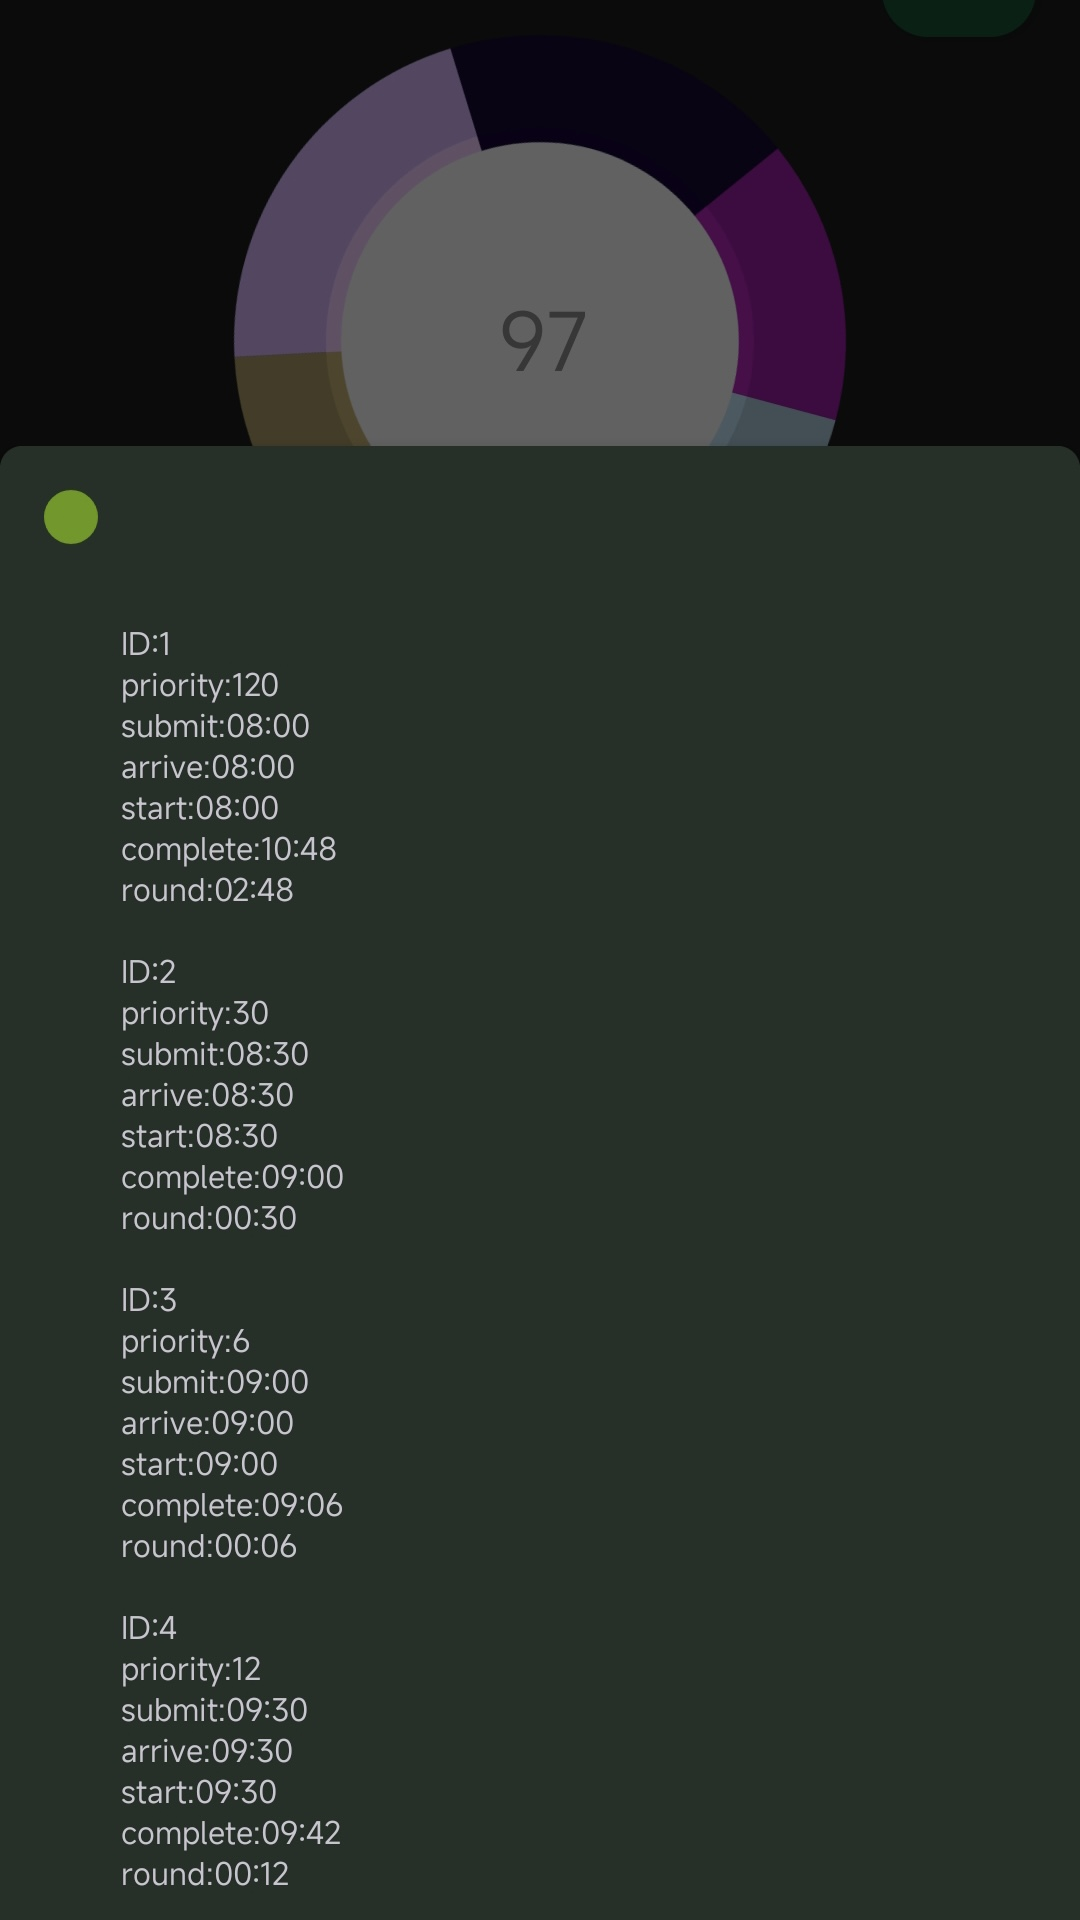
\includegraphics[width=2in]{app-timeline.jpg}
        \end{minipage}
    }
    \centering
    \caption{运行截图}
\end{figure}

\section{设计总结}

宏观来说,本次课程设计,再一次使我体验了结构化编程、面向对象程序设计的魅力。
\begin{itemize}
    \item 自顶向下,逐步求精。例如,本程序模拟处理机,接受用户输入作业序列,输出调度过程及周转时间。处理机的模拟实现可以拆分为对时钟,调度,任务的实现。调度的模拟实现可以分拆为用户提交、作业调度、进程调度、进程销毁。
    \item 抽象、封装、多态、继承。例如,各级调度虽然各司其职,分工合作,但是又有相类似行为:观察时间流逝、接受任务、移除任务、顺位排序、向上级调度提交任务等。
          正因此,本系统极大地支持扩展新的调度算法,并通过分级的形式相互排列组合。
\end{itemize}

微观地说,本次课程设计,使我有机会深入了解操作系统处理机调度的种种细节,并有机会尝试移动平台软件设计(基于Java的Android)的最佳实践。
\begin{itemize}
    \item 例如,以Activity作为Fragment的宿主,结合ViewModel(LiveData)时,需要注意ViewModelStoreOwner统一,否则无法在切片间共享数据模型。
    \item 又如,PriorityQueue结合Comparator使用,动态优先级getter/setter的tricks,深拷贝与克隆接口实现。
    \item 再如,多级反馈队列分为抢占时间片和不抢占时间片两种版本,两种的实现方式类似,唯一的区别在于更新工作队列索引的时机,所谓的“抢占”事实上是每单位时间判断(切换)一次,而所谓的“非抢占”需处理机处于“空闲”状态判断(切换)一次。
\end{itemize}

虽然本系统有一定的健壮性,可以抵御一些异常输出,但是依然存在不足,有待改进:
如不支持输入多级队列的数量(大于三个)及自定义时间片(非指数型增长),由于屏幕限制时间线界面交互设计有待改进。

\end{document}